\documentclass[11pt]{article}
% Packages
\usepackage{amsmath}
\usepackage{fullpage}
\usepackage{amsfonts}
\usepackage{amsthm}
\usepackage{graphicx}
\usepackage{hyperref}
\usepackage{geometry}
\usepackage{fancyhdr}
\usepackage{cite}
\usepackage{algorithm}
\usepackage{algorithmic}
\usepackage{pgfplots}
\usepackage{lmodern}
\pgfplotsset{compat=1.18}

% Page layout
\geometry{a4paper, margin=1in}
\setlength{\headheight}{14.49998pt}
\setlength{\headsep}{0.1in}
% Header and Footer
\pagestyle{fancy}
\fancyhf{}
\fancyhead[C]{Randomized Techniques in Graph Algorithms}
\fancyhead[R]{\thepage}

% Title
\title{Randomized Techniques in Graph Algorithms}
\author{
    Xianbang Wang\thanks{Equal Contribution} \\
    \fontsize{13}{12}\selectfont
    IIIS, Tsinghua University \\
    \fontsize{13}{12}\selectfont
    \texttt{wang-xb24@mails.tsinghua.edu.cn}
    \and
    Yiyang Lu\footnotemark[1] \\
    \fontsize{13}{12}\selectfont
    IIIS, Tsinghua University \\
    \fontsize{13}{12}\selectfont
    \texttt{luyy24@mails.tsinghua.edu.cn}
}
\date{}
\newcommand{\descendants}[1]{#1^\downarrow}
\newcommand{\ancestors}[1]{{#1}^\uparrow}
\newcommand{\cutval}[1]{{\cal C}(#1)}
\newcommand{\crossweight}[2]{{\cal C}(#1,#2)}
\theoremstyle{plain}
\newtheorem{lemma}{Lemma}[section]
\newtheorem{theorem}{Theorem}[section]
\newtheorem{definition}{Definition}[section]
\begin{document}
\maketitle
\begin{abstract}
    % This is a survey on randomized algorithms on graphs. We focus on two well-known problems: All Pairs Shortest Path (APSP) and Min Cut. We introduce the deterministic algorithms for these problems, and then present the randomized algorithms. We analyze the time complexity and success probability of the randomized algorithms, and provide experimental results. Based on the results, we discuss the practical significance of the randomized algorithms and discuss further improvements. Besides, we also discuss the application of randomized algorithms in other graph problems, such as Minimum Spanning Tree and Exact Matching. 
    
    % Inspired by the randomized algorithms, we propose a new problem: Optimal Point Traversing Path, and present a sublinear randomized algorithm to solve the special case.

    Graph algorithms are fundamental to numerous fields, providing solutions for various real-life scenarios. Traditionally, these problems have been approached with deterministic algorithms. However, randomized algorithms have emerged as powerful alternatives, capable of simplifying implementations and achieving significant performance improvements in both average-case scenarios and, sometimes, asymptotic bounds.

    In this survey, we present an in-depth exploration of randomized techniques applied to key problems in graph theory. We examine the \textbf{All Pairs Shortest Path (APSP)} problem through matrix multiplication-based approaches, analyze the \textbf{Min Cut} problem using contraction-based methods. In each case, we provide \textbf{experimental results} of both deterministic and randomized algorithms, comparing their performance and discussing possible extensions and limitations. Furthermore, we introduce randomized algorithms for the \textbf{Minimum Spanning Tree (MST)} and \textbf{Exact Matching (EM)} problems. 
    
    Inspired by the randomized algorithms, we propose a new problem: \textbf{Optimal Point Traversing Path}, and present a sublinear randomized algorithm to solve the special case, completed with a correctness proof and complexity analysis.

    Our findings highlight the advantages of randomized algorithms in terms of simplicity, speed, and scalability, while also addressing their limitations and potential applications. By including experimental results, proposing and discussing open problems, we aim to contribute both practical insights and theoretical advancements to the field of graph algorithms, encouraging further exploration of randomized methods for solving complex graph problems.
    
    All the source code used in our implementation and evaluation can be found in \url{https://github.com/PeppaKing8/algdesign-project}.

    \textbf{Keywords:} Randomized Algorithms, Graph Theory, APSP, Min Cut, MST, EM
\end{abstract}

\tableofcontents

\newpage
\section{Introduction}
\subsection{Background}\

Graph theory is an essential branch of computer science and mathematics, providing tools for solving a vast array of problems across fields such as network optimization, computational biology, logistics, and social network analysis. Many of the most widely used algorithms for solving graph-related problems - including shortest paths, minimum cuts, and spanning trees - are built on deterministic techniques, which offer robust guarantees on solution quality and are well-understood in terms of computational complexity. However, as real-world graphs grow in size and complexity, the limitations of deterministic methods become apparent, especially in scenarios where rapid, scalable solutions are required.

To address these challenges, randomized algorithms have gained prominence. By introducing randomness into the computation process, these algorithms can often achieve significant improvements in efficiency and simplicity. Randomized techniques can provide faster average-case performance, reduce algorithmic complexity, and in some cases, offer better asymptotic bounds compared to their deterministic counterparts. For example, randomized methods are particularly advantageous for large-scale or sparse graphs, where exact deterministic solutions may be computationally prohibitive.

% In particular, our contributions can be summarized as follows:
% \begin{enumerate}
%     \item All Pairs Shortest Path (APSP): We start with an overview of deterministic approaches, then delve into matrix multiplication-based methods and analyze their complexity. Extensions to directed and weighted graphs are also discussed.
%     \item Min Cut: Highlighting the Karger-Stein algorithm, we explore strategies for finding minimum cuts using contraction and fast cut techniques, and discuss improvements in data structures that can enhance efficiency.
%     \item Other Related Problems: This includes the minimum spanning tree problem, with focus on applying randomized techniques to improve runtime to linear time complexity, as well as solving exact matching problems in graphs.
%     \item Optimal Point Traversing Path: We introduce a sublinear algorithm for optimal point traversal in grid graphs, detailing its randomized components and proving its correctness.
% \end{enumerate}

% Throughout this report, we aim to demonstrate how randomness can be leveraged to solve complex graph problems more efficiently and highlight open questions and possible areas for further research in this evolving field.
\subsection{Our Work}\

This survey delves into both classic and contemporary randomized approaches for tackling fundamental graph problems. Here's an outline of our primary contributions and the structure of the survey:

\begin{enumerate}
    \item \textbf{All Pairs Shortest Path (APSP):} We begin with a review of deterministic methods for solving APSP, followed by an in-depth exploration of matrix multiplication-based algorithms. The survey examines how algorithms like APD and BPWM utilize matrix operations to reduce computational complexity. We also include a time complexity analysis and present minor enhancements to improve performance. Experimental results showcase the impact of these methods in practice, with further extensions covering directed and weighted graphs, as well as strategies for derandomization.
    \item \textbf{Min Cut:} We examine the Karger-Stein algorithm, a widely recognized randomized approach for finding minimum cuts in graphs. This section covers essential techniques, such as contraction-based methods and fast cut algorithms, and discusses their computational complexity and practical implications. Experimental results provide insights into how these techniques perform on various types of graphs, and extensions for directed and weighted graphs are proposed. We also explore the potential for improving algorithmic efficiency using advanced data structures and analyze a  $\Theta((\log n)^2)$  speedup achieved through specific optimizations.
    \item \textbf{Other Related Problems:} This section addresses the Minimum Spanning Tree (MST) and Exact Matching (EM) problems. For MST, we review classical approaches and introduce randomized algorithms that achieve linear runtime improvements. Specific topics include Borůvka's algorithm and techniques for handling light and heavy edges. The exact matching section covers the Pfaffian orientation, polynomial algorithms for calculating the Pfaffian, and randomized solutions for EM, with a focus on correctness and complexity analysis based on Schwarz's Lemma.
    \item \textbf{Our Proposed Problem:} Optimal Point Traversing Path: In addition to established problems, we propose and address an original problem focused on finding the optimal traversing path in a point-based grid graph. For this special case, we present a novel sublinear randomized algorithm, detailing its lower bounds, correctness proof, and time complexity. We conclude with a discussion on generalizing this method for broader applications beyond grid graphs.
\end{enumerate}

First two part of this survey includes experimental evaluations to compare the performance of deterministic and randomized approaches, along with a detailed analysis of the algorithms' strengths and weaknesses. By addressing these classic problems through the lens of randomized techniques, our goal is to provide valuable insights and highlight open questions in graph algorithms, ultimately advancing the understanding of where and how randomness can most effectively be applied in this field.

\section{APSP: All Pairs Shortest Path}
\subsection{Introduction}\

One of the well-known result in randomized algorithms in graph theory is the algorithm for the \textbf{All Pairs Shortest Path (APSP)} problem.

Let $G(V,E)$ be an \textbf{undirected} graph, with $V=\{1,2,\cdots,n\}$ and $|E|=m$. Let the adjacency matrix of $G$ be $A$, where $A_{ij}=A_{ji}=1$ if $(i,j)\in E$ and $A_{ij}=A_{ji}=0$ otherwise. There is a weak version of the APSP problem, \textbf{All Pairs Distance (APD)} problem, which is to compute the distance between all pairs of vertices in $G$, i.e., derive the \emph{distance matrix} $D$ where $D_{ij}$ is the length of the shortest path between $i$ and $j$.

The requirement of APSP is stronger: it requires the algorithm to compute the shortest path itself, not just the length of the shortest path, of all pairs of vertices in $G$. 

If $G$ is not connected, we can separate $G$ into connected components and solve the APSP problem for each connected component (finding connected components is easy and can be done in linear time). So we assume $G$ is \textbf{connected} in the following discussion.

Note that, if we want to store all the shortest paths, the space complexity can be $\Omega(n^3)$ (e.g. a path), which limits the time complexity we can achieve. However, we can record an \emph{implicit} representation of the shortest path - the \textbf{successor matrix} $S$: for every $(u,v)\in V^2$, let $S_{uv}$ be the vertex that is the immediate successor of $u$ on the shortest path from $u$ to $v$. This can be stored in $O(n^2)$ space, and the shortest path from $u$ to $v$ can be reconstructed by following the path $u\to S_{uv}\to S_{S_{uv}v}\to\cdots\to v$ in $O(L)$ time, where $L$ is the length of the shortest path.

\subsection{Quick Review on Deterministic Algorithms}\

The most well-known algorithm for APSP is the \textbf{Floyd-Warshall} algorithm, which has a time complexity of $O(n^3)$. The algorithm is based on dynamic programming, and the key idea is to consider all vertices as potential intermediate vertices in the shortest path. The algorithm is simple and easy to implement.

Another algorithm is based on \textbf{breadth-first search (BFS)}: for every vertex $v$, run a BFS starting from $v$ to compute the shortest path from $v$ to all other vertices. This algorithm has a time complexity of $O(nm)$, which is better when $m=o(n^2)$.

For weighted graph (every edge has a weight), the \textbf{Johnson} algorithm can be used to solve the APSP problem. The time complexity can achieve $O(nm+n^2\log n)$ using Fibonacci heap. This algorithm is an extension of Dijkstra's algorithm, which is only applicable in non-negative weight circumstance. 

It is clear that the best time complexity we can achieve for APSP is $\Omega(n^2)$, since we need to output $n^2$ shortest paths. And we also believe that $O(nm)$ is still far away from the best, especially if $m=\Omega(n^2)$.

\subsection{Matrix Multiplication-based Algorithm}\

Now we introduce a randomized algorithm for APSP, which is based on matrix multiplication. The algorithm is proposed by Alon, Galil, and Margalit in 1997\cite{alon1997exponent}.

\subsubsection{Skim on Matrix Multiplication}\

Given two $n\times n$ matrices $A$ and $B$, the product $C=AB$ is defined as $C_{ij}=\sum_{k=1}^n A_{ik}B_{kj}$. The naive algorithm has a time complexity of $O(n^3)$. The lower bound of matrix multiplication is obviously $\Omega(n^2)$, and computer scientists have been trying to find a better exponent $2<\alpha<3$ until now.

Strassen proposed a divide-and-conquer algorithm in 1969, which has a time complexity of $O(n^{\log_2 7})\approx O(n^{2.81})$. Strassen's algorithm is proved to be useful in real-life applications \cite{cite-key}, and can be parallelized to further improve performance \cite{CHOU199549}. At present, the best peer-reviewed matrix multiplication algorithm is proposed by Josh Alman, Ran Duan, Virginia Vassilevska Williams, Yinzhan Xu, Zixuan Xu and Renfei Zhou. The algorithm has a time complexity of $O(n^{2.371339})$\cite{alman2024more}. It is still an open problem to find a matrix multiplication algorithm with complexity $O(n^{2+o(1)})$, or prove that such an algorithm does not exist.
% According to Wikipedia, as of January 2024, the best peer-reviewed matrix multiplication algorithm is proposed by Virginia Vassilevska Williams, Yinzhan Xu, Zixuan Xu, and Renfei Zhou, and has complexity $O(n^{2.371552})$ \cite{williams2023newboundsmatrixmultiplication}. 

\emph{From now on, suppose we have a matrix multiplication algorithm with time complexity $O(n^\nu)$.}

\subsubsection{APD}\

Recall that $A$ is adjacency matrix. Let $\bar{A}$ be the matrix where $\bar{A}_{ij}=1$ if $i=j$ or $A_{ij}=1$. The connection between the shortest path and matrix multiplication is revealed by the following lemma.
\begin{lemma}
    \label{lemma:shortest_path_matrix_multiplication}
    Let $k$ be a positive integer. For every $i,j\in V$, $D_{ij}\le k$ if and only if $\bar{A}^k_{ij}>0$.
\end{lemma}
\begin{proof}
If $\bar{A}^k_{ij}>0$, considering the procedure of matrix multiplication, there must be $i_0=i,i_1,i_2,\cdots,i_k=j\in V$, such that $\bar A_{i_0i_1}=\bar A_{i_1i_2}=\cdots=\bar A_{i_{k-1}i_k}=1$. So there is a path $i_0\to i_1\to i_2\to\cdots\to i_k$ of length $k$ from $i$ to $j$, which implies $D_{ij}\le k$.
\end{proof}

The lemma implies that we can compute the distance matrix $D$ by computing $\bar{A}^k$ for $k=1,2,\cdots,n$. However, this requires $O(n^{\nu+1})=\omega(n^3)$ time, which is even worse.

The idea to improve this is: we compute $\bar A^2$, which can reduce the length of the shortest path to a half, and do the computation recursively. We should first get $A'$, where $A'_{ij}=1$ if $A_{ij}=1$ or there is a path of length 2 from $i$ to $j$. From Lemma \ref{lemma:shortest_path_matrix_multiplication}, we can derive $A'$ from $\bar A^2$ in $O(n^2)$: $A'_{ij}=1$ if and only if $\bar A_{ij}>0$.

Recursively run the algorithm on $A'$ (which also represents a graph $G'$), and suppose we got a distance matrix $D'$ for $G'$. Now we want to retrieve $D$.

\begin{lemma}
\label{2}
For every $i,j\in V$, $D'_{ij}=\lceil\dfrac{D_{ij}}{2}\rceil$.
\end{lemma}
\begin{proof}
Due to the definition of $A'$, $D'$ represents the distance, where we can walk 2 steps at a time. The lemma is then obvious.
\end{proof}

Lemma \ref{2} is inadequate because given $D'$, every element of $D$ has two choices. However, Lemma \ref{3} could tell us the answer.
\begin{lemma}
\label{3}
Let $i\not=j \in V$. For any neighbor $u$ of $i$ in $G'$, $D_{ij}-1\le D_{uj}\le D_{ij}+1$. And there exists at least one $u$, such that $D_{uj}=D_{ij}-1$.
\end{lemma}
\begin{proof}
For any neighbor $u$, we can first go to $i$, and walk $D_{ij}$ steps to $j$. Thus, there is a path from $u$ to $j$ of length $D_{ij}+1$, implying $D_{uj}\le D_{ij}+1$. Interchange $i$ and $u$, we can get $D_{uj}\ge D_{ij}-1$. Suppose the shortest path between $i,j$ is $i\to i_1\to\cdots\to i_t=j$, then $D_{i_1j}=D_{ij}-1$.
\end{proof}

\begin{lemma}
\label{4}
If $D_{ij}$ is even, $D'_{kj}\ge D'_{ij}$ for every neighbor $k$ of $i$; if $D_{ij}$ is odd, $D'_{kj}\le D'_{ij}$ for every neighbor $k$ of $i$, and at least one equality does not hold.
\end{lemma}
\begin{proof}
Suppose $D_{ij}=2t$ is even. Lemma \ref{3} tells $D_{kj}\in\{2t-1,2t,2t+1\}$ for every neighbor $k$ of $i$. Use Lemma \ref{2}, $D'_{kj}\ge t=D'_{ij}$. \\
Now suppose $D_{ij}=2t+1$ is odd, then $D_{kj}=\{2t,2t+1,2t+2\}$, so $D'_{kj}\in \{t,t+1\}$, thereby $\le t+1=D'_{ij}$. And at least one $k$ satisfies $D_{kj}=D_{ij}-1=2t$, so $D'_{kj}=t<D'_{ij}$.
\end{proof}

In fact, to compute $D$ from $D'$, we only need to know the parity of each $D_{ij}$. From Lemma \ref{4}, we can separate even and odd $D_{ij}$, and compute $D$ in $O(n^2)$ time. Specifically, $D_{ij}$ is even if and only if
$$\sum\limits_{k\text{ is neighbor of }i} D'_{kj}\ge d_iD_{ij},$$
$d_i$ is the degree of $i$. If $S=AD'$, then $D_{ij}$ is even if and only if $S_{ij}\ge d_iD_{ij}=\bar A^2_{ii}D_{ij}$. The implementation is shown in Algorithm \ref{alg:example}.

\begin{algorithm}
\caption{APD}
\label{alg:example}
\begin{algorithmic}[1]
    \STATE \textbf{Input:} Graph $G=(V,E)$ with adjacency matrix $A$
    \STATE \textbf{Output:} Distance matrix $D$
    \STATE $\bar A\leftarrow I+A$
    \STATE $A^*\leftarrow \bar A^2$
    \FOR{$i=1$ to $n$}
        \FOR{$j=1$ to $n$}
            \STATE $A'_{ij}\leftarrow 1$ if $A_{ij}=1$ or ${A^*}_{ij}>0$
        \ENDFOR
    \ENDFOR
    \STATE $D'\leftarrow$ APD$(A')$
    \STATE $S\leftarrow AD'$
    \FOR{$i=1$ to $n$}
        \FOR{$j=1$ to $n$}
            \STATE $D_{ij}\leftarrow 2D'_{ij}$ if $S_{ij}\ge A^*_{ii}D'_{ij}$, otherwise $D_{ij}\leftarrow 2D'_{ij}-1$
        \ENDFOR
    \ENDFOR
    \RETURN $D$
\end{algorithmic}
\end{algorithm}

\subsubsection{APSP}\

Observe that, the preceding algorithm does not provide enough information of successor matrix $S$. More precisely, if $D_{ij}$ is even, it is not guaranteed from Lemma \ref{4} that we can find $k$ just from $D'$.

Suppose $D$ is computed with algorithm \ref{alg:example}. For every $i,j\in V$, how to find $S_{ij}$? Or, what is the necessary and sufficient condition of $S_{ij}$? The answer of the last question is clear: $(i,S_{ij})\in E$, and $D_{ij}-1 = D_{S_{ij}j}$. Let $r=D_{ij}$. For every integer $u\ge 0$, define $D^{(u)}$ as: $D^{(u)}_{ij}=1$ iff $D_{ij}=u$. So $S_{ij}$ is one of the \textbf{witness} of $A$ and $D^{(r-1)}$ w.r.t $i,j$. (\emph{Note: the witness of two matrices $A$ and $B$ w.r.t. $i,j$ is an index $x$ that $A_{ix}=B_{xj}=1$.})

Given two 0-1 matrices $A,B$, to compute a \textbf{witness matrix} is a well-known problem in computer science called \textbf{Boolean Product Witness Matrix (BPWM)}. We will leave the implementation of BPWM in section \ref{sec:bpwm}. Now assume we have a black box $\mathbf{BPWM}(A,B)$.

From the above discussion, we need to enumerate $r=1,2,\cdots,n$ and compute $D^{(r-1)}$ for each $r$, and derive the witness matrix of $A$ and $D^{(r-1)}$, which needs $O(n)$ times of $\mathbf{BPWM}$. However, a clever optimization can reduce to only $3$ times. For $s=0,1,2$, Let $D^{[s]}$ be the matrix where $D^{[s]}_{ij}=1$ iff $D_{ij}\equiv s\pmod 3$. Denote the witness of $A$ and $D^{[s]}$ by $W^{[s]}$.

\begin{lemma}
\label{5}
For every $i,j\in V$, $S_{ij}=W^{[(D_{ij}-1)\mod 3]}_{ij}$.
\end{lemma}
\begin{proof}
Firstly, $S_{ij}$ is a witness of $A$ and $W^{[(D_{ij}-1)\mod 3]}$. This is because $(i,S_{ij})\in E$, and $D_{S_{ij}j}=D_{ij}-1$, thereby also $\equiv D_{ij}-1\pmod 3$. Note that this also implies that $W^{[(D_{ij}-1)\mod 3]}_{ij}$ exists.\\
On the other hand, suppose $v=W^{[(D_{ij}-1)\mod 3]}_{ij}$. Then $D_{vj}\equiv D_{ij}-1\pmod 3$, and $v$ is a neighbor of $i$. Since from Lemma \ref{3}, $D_{vj}\in [D_{ij}-1,D_{ij}+1]$, we immediately get $D_{vj}=D_{ij}-1$, which means $v$ is one of the successor.
\end{proof}

Thus, if $W^{[s]}(s=0,1,2)$ is computed, $S$ can be derived in $O(n^2)$ time. The time complexity is $O(f(n)+n^2)$, where $f(n)$ is the time complexity of \textbf{BPWM}, obviously $\Omega(n^2)$.

\subsubsection{BPWM}
\label{sec:bpwm}\

Recall that the input of BPWM is two 0-1 $n\times n$ matrices $A,B$, and the output is a matrix $W$, where $W_{ij}$ is the witness of $A$ and $B$ w.r.t. $i,j$.

Consider a simple case: assume for every $i,j$, the witness is \textbf{unique}. Define weighted matrix $A^{\#}$ as: $A^{\#}_{ik}=kA_{ik}$. Now, we compute $W^{\#}=A^{\#}B$. Since $A^{\#}$ is weighted - intuitively, the vertex $i$ has value $i$. From the definition of $W^{\#}$, $W^{\#}_{ij}$ is the sum of the values of all the witnesses. Since the witness is unique, $W^{\#}_{ij}$ is the value of the witness. So we can derive $W$ from $W^{\#}$ in $O(n^2)$ time - $W=W^{\#}$, actually.

Now consider the general case. We continue to use the ``weighted'' idea, but just choose a \textbf{subset} of $V$ to be the weighted. If we are lucky, the witness is unique within the subset, and we are done. We will see that randomization give us that luck.

For every $i,j$, suppose there are $t$ witnesses. From easy math, there exists a positive integer $r$, such that $\dfrac{n}{2}\le tr\le n$. Randomly choose a subset of rank $r$ of $V$, and weight them with their own index. For other $n-r$ vertices, weight them with $0$. The following lemma shows the probability of choosing a unique witness is larger than a positive constant!

\begin{lemma}
\label{6}
Let $v=\{1,2,\cdots,n\}$, $S_0=\{1,\cdots,t\}$, integer $r$ satisfies $\dfrac{n}{2}\le tr\le n$. Randomly choose a subset $S\subseteq V$ of rank $r$. We have
$$P(|S\cap S_0|=1)\ge \dfrac{1}{2e}.$$
\end{lemma}
\begin{proof}
Since $tr\le n$, we have $\dfrac{r-1}{n-t}\le \dfrac{1}{t}$. The probability is
\begin{align*}
\dfrac{t\cdot \binom{n-t}{r-1}}{\binom{n}{r}} &= t\cdot \dfrac{(n-t)!r!(n-r)!}{(r-1)!(n-t-r+1)!n!}\\
&= \dfrac{tr}{n}\cdot \dfrac{(n-t)!(n-r)!}{(n-t-r+1)!(n-1)!}\\
&= \dfrac{tr}{n}\cdot \prod\limits_{i=0}^{t-2} \dfrac{n-r-i}{n-1-i}\\
&\ge \dfrac{tr}{n}\cdot \left(1-\dfrac{r-1}{n-t}\right)^{t-1}\\
&\ge \dfrac{1}{2}\cdot \left(1-\dfrac{1}{t}\right)^{t-1} \ge \dfrac{1}{2e}.
\end{align*}
\end{proof}

Lemma \ref{6} shows that, if we try $L$ different subsets, the probability to fail (i.e. in each case $|S\cup S_0|\not=1$) will be $O(\exp{\Theta(n)})$. Lemma \ref{7} shows that we can choose appropriate $r$ within a set of $O(\log n)$ candidates.

\begin{lemma}
\label{7}
For every $1\le t\le n$, there exists a natural number $k\le \log n$, such that $\dfrac{n}{2}\le t\cdot 2^k\le n$.
\end{lemma}
\begin{proof}
Let $k$ be the largest integer such that $t\cdot 2^k\le n$. Then $t\cdot 2^{k+1}>n$, so $t\cdot 2^k\le n/2$. And $2^k\le t\cdot 2^k\le n$, so $k\le \log n$, as desired.
\end{proof}

So the algorithm is as follows: enumerate every $r=1,2,\cdots,2^{\lfloor\log n\rfloor}$. For every $r$, randomly choose $L=\Theta(\log n)$ subsets of rank $r$, and compute the witness matrix. For every $i,j$, Lemma \ref{6} tells us the probability to fail is $o(\dfrac{1}{n^2})$ if $\lim\limits_{n\to \infty}\dfrac{L}{\log n}$ is sufficiently large. Then the union bound directly bounds the failing probability by $o(1)$.

If we have missed some witness (which is very unlucky), we found these missing witnesses by brute-force - $O(n)$ for every pair $(i,j)$. Since the expected number of missing pair is $O(1)$, the time complexity of this procedure can be ignored.

In practice, we set $L=\gamma\log n$, where $\gamma$ is a constant. We pick $\gamma=3$ in practice, considering the trade-off between time complexity and success probability. 

The whole algorithm (APSP) is shown in Algorithm \ref{alg:APSP}. The black box \textbf{BPWM} is implemented in Algorithm \ref{alg:BPWM}.

\begin{algorithm}
    \caption{APSP}
    \label{alg:APSP}
    \begin{algorithmic}[1]
        \STATE \textbf{Input:} Graph $G=(V,E)$ with adjacency matrix $A$
        \STATE \textbf{Output:} Successor matrix $S$
        \STATE $D\leftarrow \text{APD}(A)$
        \FOR{$s\in \{0,1,2\}$}
            \STATE compute $D^{[s]}$ by: $D^{[s]}_{ij}=1$ iff $D_{ij}\equiv s\pmod 3$
            \STATE $W^{[s]}\leftarrow \text{BPWM}(A,D^{[s]})$
        \ENDFOR
        \FOR{$i=1$ to $n$}
            \FOR{$j=1$ to $n$}
                \STATE $r\leftarrow (D_{ij}-1)\mod 3$
                \STATE $S_{ij}\leftarrow W^{[r]}_{ij}$
            \ENDFOR
        \ENDFOR
    \RETURN $S$
    \end{algorithmic}
\end{algorithm}

\begin{algorithm}
    \caption{BPWM}
    \label{alg:BPWM}
    \begin{algorithmic}[1]
        \STATE \textbf{Input:} 0-1 matrices $A,B$ of size $n\times n$
        \STATE \textbf{Output:} Witness matrix $W$
        \FOR{$t=0,1,\cdots,[\log n]$}
            \STATE $r\leftarrow 2^t$
            \FOR{$l=1$ to $\gamma\log n$}
                \STATE Randomly choose a subset $S$ of rank $r$
                \STATE construct $A^{\#}$: $A^{\#}_{ik}\leftarrow kA_{ik}$ for $i\in S$, $0$ otherwise
                \STATE $W^{\#}\leftarrow A^{\#}B$
                \FORALL{$(i,j)$}
                    \STATE $W_{ij}\leftarrow W^{\#}_{ij}$ if $W_{ij}$ is not defined and $W^{\#}_{ij}$ is a witness
                \ENDFOR
            \ENDFOR
        \ENDFOR
        \FORALL{$(i,j)$}
            \IF{$W_{ij}$ is not defined}
                \STATE $W_{ij}\leftarrow$ brute-force to find the witness
            \ENDIF
        \ENDFOR
    \RETURN $W$
    \end{algorithmic}
\end{algorithm}

\subsubsection{Time Complexity Analysis}

\paragraph{APD} APD is a deterministic algorithm and it performs recursively. Since every recursion we reduce the length of the shortest path by a half, the depth of the recursion is $O(\log n)$. In every recursion, we need to compute $A^*$ and $S$, which takes $O(n^{\nu})$ time (recall that this is the hypothesized time complexity of matrix multiplication). Other procedures just take $O(n^2)=o(n^{\nu})$ time. So the time complexity of APD is $O(n^{\nu}\log n)$.

\paragraph{BPWM} Consider $(t,l)$, we have $O(\log n\cdot \log n)=O(\log^2 n)$ pairs. For every pair, we need to compute $W^{\#}$, which takes $O(n^{\nu})$ time. Other procedures take $O(n^2)$ time. So the time complexity of BPWM is $O(n^{\nu}\log^2 n)$.

\paragraph{APSP} APSP \ref{alg:APSP} calls APD \ref{alg:example} and BPWM \ref{alg:BPWM} for constant times, so the time complexity is $O(n^{\nu}\log^2 n)$.

\subsubsection{Small Improvement}
\label{imp}\

Using careful analysis, we can actually show that BPWM is $O(n^\nu \log n)$, so APSP is also $O(n^\nu \log n)$. The key idea is, $A^\#$ can be reduced to $n\times r$, so $W^\#$ is actually multiplication of two matrices of size $n\times r$ and $r\times n$ respectively.

For matrix of size $n\times r$, divide it into $\lfloor\dfrac{n}{r}\rfloor$ blocks (by row). For $r\times n$ matrix is similar. Then we can compute each pair of blocks in $O(r^{\nu})$ time, and combine them into one single $n\times n$ matrix in $O(n^2)$ time. So the time complexity of this multiplication is $O(r^\nu(\dfrac{n}{r})^2)=O(r^{\nu-2}n^2)$.

So, the time complexity of BPWM is
\begin{align*}
\sum\limits_{t=0}^{\log n}\sum\limits_{l=1}^{\gamma\log n} O(r^{\nu-2}n^2) &= \gamma\log n\cdot \sum\limits_{t=0}^{\log n} O(r^{\nu-2}n^2)\\
&= \gamma\log n\cdot O(n^2)\cdot \sum\limits_{t=0}^{\log n} O(2^{t(\nu-2)})\\
&= \gamma\log n\cdot O(n^2)\cdot O(n^{\nu-2}) = O(n^\nu\log n)
\end{align*}
if $\nu>2$.

\subsection{Experimental Results}\

We implemented four algorithms for APSP: for the deterministic algorithms, we implemented Floyd-Warshall and BFS; for the randomized algorithms, we implemented the matrix multiplication-based algorithm with two versions: one with Strassen's algorithm and the other with the trivial matrix multiplication. The latter two is the improved version of the algorithm in section \ref{imp}.

Algorithms are implemented with C++.

\subsubsection{Settings}\

We set the graph size to be $n=2^k$, where $k\le 8$. In our experiment, edges are independently and uniformly generated, each with probability $p$. To ensure the graph is connected, after graph is randomly generated, we add $M-1$ edges to connect the graph, where $M$ is the number of connected components.

Our test environment is $\texttt{-std=C++11}$ and has unlimited stack size. 

\subsubsection{Parameters}\

We set $\gamma=3$ in BPWM, and the threshold of Strassen's algorithm to be $n_0=64$. $p=0.1$ since we do not want the graph to be too dense, and also limit the performance of BFS.

\subsubsection{Results}\

We run the algorithms for 5 times and record the average execution time. The results of $k=7,8$ ($n=128,256$) are shown in Figure \ref{fig:et}. 

An interesting phenomenon is, when $k$ increase by 1, the execution time of \texttt{BFS} and \texttt{Floyd} increase by a factor of $3\sim 4$, while the execution time of \texttt{Strassen} and \texttt{Trivial} increase by a factor of $5\sim 6$. This is partially due to the optimization of C++ compiler, which can optimize the loops in \texttt{BFS} and \texttt{Floyd} to be more cache-friendly - but not the case when there are heavy matrix multiplications.

\begin{figure}[ht]
    \centering
    \begin{tikzpicture}
        \begin{axis}[
            ybar,
            bar width=0.3cm,
            width=0.8\textwidth,
            height=0.5\textwidth,
            symbolic x coords={BFS, Floyd, Trivial, Strassen},
            xtick=data,
            ylabel={Execution Time (ms)},
            xlabel={Algorithms},
            ymin=0,
            ymax=3000,
            legend style={at={(0.5,-0.15)}, anchor=north, legend columns=-1},
            nodes near coords,
            enlarge x limits={abs=0.75cm}
        ]
        \addplot coordinates {(BFS, 159) (Floyd, 151) (Trivial, 467) (Strassen, 428)};
        \addplot coordinates {(BFS, 428) (Floyd, 510) (Trivial, 2479) (Strassen, 2245)};
        \legend{$k=7$, $k=8$}
        \end{axis}
    \end{tikzpicture}
    \caption{Execution time of different algorithms on two datasets}
    \label{fig:et}
\end{figure}

\subsubsection{Analysis}\

Granted, although the time complexity of \texttt{Strassen} is better than \texttt{BFS} and \texttt{Floyd}, the actual execution time is much larger. This is because the constant factor of Strassen's algorithm is remarkably large. Moreover, if the parameter is not carefully chosen, or $p$ is much smaller, \texttt{BFS} will perform even better and \texttt{Strassen} and \texttt{Trivial} will be even worse. Consequently, the matrix multiplication-based algorithm has less practical significance than theoretical significance.

Based on the data of $k=8$, we can approximate the constant factor of these algorithms. Suppose the execution time of \texttt{Floyd} is $\beta\cdot n^3$, and the execution time of \texttt{Strassen} is $\alpha\cdot n^{\log_2 7}\log n$. Plugging in the data, we can get $\alpha\approx 3.9\cdot 10^{-4}$ and $\beta\approx 8.5\cdot 10^{-5}$. Finding the threshold $N$, which satisfies $\alpha\cdot N^{\log_2 7}\log N=\beta\cdot N^3$, we can get $N\approx 2500$. 

Since for $n=2^k$, Strassen's algorithm is much faster than other cases (which need to expand the matrix up to $4$ times of parameters), we can extrapolate that the actual threshold should be $N_0\approx 10^4$. \texttt{Strassen} will likely be faster than \texttt{Floyd} when $n\gg N_0$; if we replace Strassen's matrix multiplication with the most advanced algorithm, we surmise that the threshold will be slightly lower.

\subsection{Extensions}

\subsubsection{Derandomization}\

One of the popular method for \textbf{derandomization} is \textit{pseudo-randomness}. With generating pseudo-random bits from a random source, we may simulate the randomized algorithm deterministically, without having the change of trying all possible bits - because a relatively small subset of bits can ensure the pseudo-randomness.

Notice that the random part in APSP is the calculation of witness matrix. \cite{267748} shows that we can derandomize the process. 

First we consider an alternative approach to BPWM. The idea is, we randomly delete some entries in $B$ iteratively, and in each iteration, we check if some witnesses are easy to compute. Specifically, we maintain an $0-1$ matrix $R$: at first it is $J$ (all entries are $1$), and in each iteration we cover some entries of $R$ with $0$, and calculate $A\cdot (B\land R)$. The sketch of the algorithm is shown in Algorithm \ref{alg:bp2}.

\begin{algorithm}
    \caption{An Alternative BPWM Algorithm}
    \label{alg:bp2}
    \begin{algorithmic}[1]
        \STATE \textbf{Input:} 0-1 matrices $A,B$ of size $n\times n$
        \STATE \textbf{Output:} Witness matrix $W$
        \STATE $C\leftarrow AB$
        \STATE While not all witnesses are computed
            \STATE\quad Let $L$ be positive entries of $C$ that have no witness yet
            \STATE\quad Initialize $R\leftarrow J$
            \STATE\quad Repeat $\lceil1+3\log_{4/3}n\rceil$ times
                \STATE\quad\quad i.\ $D\leftarrow A\cdot (B\land R)$
                \STATE\quad\quad ii.\ $L'\leftarrow$ all entries of $D$ in $L$ that are at most $c$
                \STATE\quad\quad iii.\ Find all witnesses in $L'$
                \STATE\quad\quad iv.\ $R\leftarrow R'$ satisfying two conditions
    \RETURN $W$
    \end{algorithmic}
\end{algorithm}

In step iv, the two conditions are: (I)\ denote $D'=A\cdot (B\land R')$, then the sum of all entries in $D'$ is at most $3/4$ of which in $D$; (II)\ the fraction of entries of $D$ in $L$ that greater than $c$ but the corresponding entries in $D'$ are $0$ is at most $\alpha$.

If (I) holds, since the sum of all entries in $A\cdot B$ is at most $n^3$, with $\ge 1+3\log_{4/3} n$ iterations, all entries of $R$ will vanish. That explains the repeat time parameter.

Let $S$ be a random $0-1$ matrix. We will now show that, there is a remarkable possibility that, $R':=R\land S$ satisfies (I) and (II) both - if we choose $c$ and $\alpha$ properly.

\begin{lemma}
\label{apspext1}
The probability that (I) holds is at least $1/3$.
\end{lemma}

\begin{proof}
For every $(i,k,j)$ such that $A_{ik}=B_{kj}=R_{kj}=1$, the probability of this pair to vanish in the calculation of $D'$ is exactly $1/2$ (due to the randomness of $S$). Using Markov's inequality we get the result.
\end{proof}

\begin{lemma}
\label{apspext2}
The probability that (II) holds is at least $\dfrac{1}{2^c\alpha}$.
\end{lemma}

\begin{proof}
First consider every entry $D_{ij}>c$. If $D'_{ij}=0$, it means that every entry in $B\land R$ that contributes to $D_{ij}$ should be eliminated. Thus, the probability is at most $\dfrac{1}{2^c}$. Using Markov's inequality we get the result.
\end{proof}

If $c,\alpha$ is chosen such that $\dfrac{1}{2^c\alpha}<C<\dfrac{1}{3}$ where $C$ is constant, we will have a constant positive possibility to success ($\dfrac{1}{3}-C$, using union bound). Since to verify two conditions are just about one multiplication and an $O(n^2)$ time check, $\tilde O(n^\nu)$ will be used in expectation at step iv. 

Now we will prove that: in the ``while not all witnesses are computed'' part, we will do at most $\tilde O(1)$ times. It is ensured by the condition (II), as we will show in Lemma \ref{apspext3}.

\begin{lemma}
\label{apspext3}
In each iteration, at least $(1-\alpha)^{M}$ fraction of entries of $D$ in $L$ will be given an witness, where $M=1+3\log_{4/3} n$.
\end{lemma}

\begin{proof}
Since (II) is satisfied in each update of $R$, only $\le \alpha$ fraction of \textbf{new} entries will not be considered in step ii. So at least $1-\alpha$ fraction is still under consideration. The lemma follows since $M$ is the max repeat time.
\end{proof}

If $(1-\alpha)^M$ is also greater than a positive constant, we are done. In fact, we can choose $c\sim\log \log n$ and $\alpha=\dfrac{1}{2^{c-3}}$. It is easy to verify $\dfrac{1}{2^c\alpha}=\dfrac{1}{8}<\dfrac{1}{3}$ and $(1-\alpha)^M>\exp\{-3\}>0$.

Here comes the pseudo-random part. Notice that the randomness of $S$ is only used in a subset of size $c$ in Lemma \ref{apspext1} and \ref{apspext2}. Can we find a \textbf{very small} subset $\mathcal{S}$ of $\{0,1\}^n$ such that, if we look to every $I\subseteq\{1,2,\cdots,n\}$ and $|I|=t\le c$, elements in $\mathcal{S}$ restricted to $I$ is enough random (every $2^t$ possibilities appear with \textbf{almost equal} probability)? For ``almost'', we mean there is a very small $\epsilon>0$ s.t. for every possibility $P$, the probability of $P$ is in $[2^{-t}-\epsilon,2^{-t}+\epsilon]$. The termination of this condition is \underline{$c$-wise $\epsilon$-dependent.}

Suppose $\epsilon=\dfrac{1}{2^{c+1}}$. We have alternative lemmas of Lemma \ref{apspext1} and \ref{apspext2}, if $S$ is randomly picked in $\mathcal{S}$:

\begin{lemma}
\label{apspext4}
The probability that (I) is satisfied is at least $\dfrac{1}{3}-2\epsilon$; for (II), it is $(\dfrac{1}{2^c}+\epsilon)\cdot \alpha^{-1}$.
\end{lemma}

\begin{proof}
The proof of the first one is similar to Lemma \ref{apspext1} - just change the expectation to $1/2+\epsilon$. For the second one, observe that for each $D_{ij}>c$, pick an arbitrary subset of witnesses of $(i,j)$ with rank $c$ and use the pseudo-randomness hypothesis - we only need to change $1/2^c$ into $1/2^c+\epsilon$.
\end{proof}

Using union bound, we can prove that the probability of one-shot success is at least $1/12-2\epsilon$. As shown in \cite{10.1145/100216.100244}, we can construct a $c$-wise $\epsilon$-dependent set $\mathcal{S}$ with size
$$(\log n\cdot\dfrac{c}{\epsilon})^{2+o(1)}=\tilde O(1).$$
So the ``random generation'' of $S$ can be replaced by trying every possible set in $\mathcal{S}$ one-by-one. Note that this also explains how to do step iii: with pseudo-randomness, for every entry that is selected in step ii, there exists $S'\in \mathcal{S}$ such that only one witness is preserved. As we have shown above, we can use another one matrix multiplication to find indices of these entries. In other words, we do iii and iv simultaneously.

For the deterministic construction of $\mathcal{S}$, please refer to \cite{10.1145/100216.100244}. Here we provide an theoretical proof that such subset of this size exists:

\begin{lemma}
\label{psr1}
Suppose $c\ge 5$, $\epsilon=\dfrac{1}{2^{c+1}}$, $M=(\log n\cdot 2^{c+10})^2$. Then there exists a $c$-wise $\epsilon$-dependent set $\mathcal{S}$ of size $M$.
\end{lemma}

\begin{proof}
Let every element in $\mathcal{S}$ be randomly chosen. We will prove that the probability that $\mathcal{S}$ is not $c$-wise $\epsilon$-dependent is less than $1$, which means there exists a set that satisfies the condition. Fix a subset $T$ of size $c$. The number of elements in $\mathcal{S}$ that have $(0,\cdots,0)$ in $T$, $k$, is sampled from $\text{Binomial}(M,2^{-c})$. Using Hoeffding's inequality, we have
$$P(|k-\dfrac{M}{2^{c}}|>M\cdot \epsilon) \le \exp\{-2\epsilon^2 M\}.$$
Applying union bound, the probability to fail is at most
$$\exp\{-2\epsilon^2 M\}\cdot 2^c\cdot \dbinom{n}{c}\le \exp\{-2\epsilon^2M\}2^n/\epsilon.$$
In order to let RHS smaller than $1$, we only need to have
$$M\ge \dfrac{\log n-\log \epsilon}{2\epsilon^2}=(\log n+2c)2^{2c+1}\le (\log n\cdot 2^{c+10})^2,$$
finishing the proof.
\end{proof}

\subsubsection{Directed Graph and Weighted Graph}\

We may have noticed that, the above algorithm applies only on unweighted graph. Which means, all weights in the graph must be 1. However, similar methods can be used to compute APSP in more general graphs. \cite{ALON1997255} devised an $O(n^{(3+\nu)/2}\log^3 n)$ algorithm to compute APSP($n,1$) - where every weight of an edge is $-1,0$, or $1$. For APSP($n,M$) ($|w|\le M$ for every weight $w$), we can simply expand every edge into $M$ edges, yielding an algorithm of time complexity $O(n^{(3+\nu)/2}M^{(3+\nu)/2}(\log^3 n+\log^3 M)).$

For (unweighted) directed graph, \cite{zwick2000pairsshortestpathsusing} designed an algorithm, also based on matrix multiplication, that runs in $\tilde O(n^{2+1/(4-\nu)})$ time.

\subsection{Open Problems}\

An open problem is to further improve the time complexity for computing witness matrix. For instance, can we find a BPWM method that is $O(n^\nu)$? Alternatively, several open problems are still focusing on improving the best algorithms for $APSP(n, M)$, for directed or undirected graphs by improving the exponent or by improving the dependence on $M$.

Furthermore, given the shortest distances, how hard is it to compute witnesses for the shortest paths? Possibly, this can be solved in $O(n^2)$ time, but all algorithms either need additional matrix multiplications or have a higher time complexity. \cite{alon1997exponent}

Still, computer scientists do not know whether there exists an APSP algorithm, either deterministic or randomized, that is $O(n^2)$. No stronger lower bound is proved - since this implies a stronger lower bound for matrix multiplication.
\section{Min Cut}

\subsection{Introduction}\

\textbf{Min Cut} problem is a well-known problem in graph theory. The problem is defined as follows: 
\begin{definition}
    Given a  undirected graph $G(V,E)$, with $V=\{1,2,\cdots,n\}$ and $|E|=m$, define the adjacency matrix $A$, where $A_{ij}=A_{ji}=1$ if $(i,j)\in E$ and $A_{ij}=A_{ji}=0$ otherwise. A \textbf{cut} of $G$ is a partition of $V$ into two sets $S$ and $V\backslash S$, where $S\neq\emptyset$ and $V\backslash S\neq\emptyset$. The \textbf{cost} of a cut $(S,V\backslash S)$ is defined as
    \begin{align*}
        \text{cost}(S,V\backslash S)=\sum_{i\in S, j\in V\backslash S}A_{ij}
    \end{align*}
    The Min Cut problem is to find a cut $(S,V\backslash S)$ with the minimum cost.
\end{definition}

The Min Cut problem has a wide range of applications in computer science, such as image segmentation, clustering, network reliability, etc. The problem is also a fundamental problem in graph theory, and has been studied for decades. Variations of the minimum cut problem consider weighted graphs, directed graphs, terminals, and partitioning the vertices into more than two sets.

\subsection{Quick Review on Deterministic Algorithms}\

Deterministic algorithms for minimum cut problem are initially derived from minimum $s-t$ cut problem, which aims to find a partition that separates $s$ and $t$ and minimizes the weight between the edges. It's well known that 
\begin{lemma}
    In a undirected graph $G(V,E)$, given two vertices $s,t\in V$, the minimum $s-t$ cut equals the maximum $s-t$ flow.
\end{lemma}
To find the global minimum cut, a naive thought is executing maximum flow algorithm for $s=0,t=1,\cdots,n-1$, which has a time complexity of $O(n\text{MF}(n,m))$, where $\text{MF}(n,m)$ is the time complexity of maximum flow algorithm. Since the best deterministic maximum flow problem runs in time $O(mn\log(n^2/m))$, using this naive approach would require $\Omega(n^2m)$. 

Fortunately, using \textbf{Stoer-Wagner}\cite{stoer1997simple} algorithm, the $n-1$ maximum flow computations can be implemented in the time proportional to the cost of a single maximum flow, which has a time complexity of $O(nm+n^2\log n)$. 

Using a more sophisticated algorithm, we can achieve a lower time complexity. In 2024, the \textbf{SOTA}\cite{doi:10.1137/1.9781611977912.111} of deterministic algorithm of Min Cut runs in $\tilde{O}(n^2)$ time, which is near optimal (since the input size is $\Omega(n+m)$, which is $\Omega(n^2)$ in the worst case).

The computation model introduced above is based on \textbf{Sequential Model}, which is standard unit-cost RAM model. Besides, there are more computation models of Min Cut and corresponding SOTA\footnote{The statistics here consider randomized algorithm and corresponding complexity requires high probability.} as following:
\begin{enumerate}
    \item \textbf{Cut Query}: Allowed to query arbitrary cuts of $G$, charged once for each query. The SOTA is $\tilde{O}(n^2)$\cite{mukhopadhyay2020weighted}.
    \item \textbf{Parallel RAM}: Concurrent read exclusive write PRAM model. The complexity consists of time complexity and work complexity, where work complexity equals to the sum of time complexity of all processors. The SOTA is $O(m\log n)$ work and $O(\log^3 n)$ time\cite{anderson2023parallel}.
    \item \textbf{Dynamic semi-streaming}: Allowed using $O(n\text{poly}\log n)$ bits of internal memory, which is charged once per pass. The SOTA is using 2 passes with $O(n\log n)$ bits of memory\cite{assadi2021simple}.
    \item \textbf{Distributed CONGEST}: You can only communicate with neighbors in a synchronous network. The bandwidth is restricted with $O(\log n)$ bits per round. The complexity charged once per round. The SOTA is $\tilde{O}(\sqrt{n}+D)$ rounds for graph with diameter $D$\cite{dory2021distributed}.
\end{enumerate}

In this survey, we will focus on the Sequential Model since it is the most common computation model in practice. We will introduce the randomized algorithms of Min Cut based on this.

\subsection{Karger-Stein Algorithm}\

Now we introduce a randomized algorithm for Min Cut, which is based on Karger's algorithm\cite{inproceedings}. The algorithm is proposed by Karger and Stein in 1996\cite{karger1996new}.

The randomized algorithm of Min Cut is a \textbf{Monte Carlo} algorithm, which means that the algorithm may output a wrong answer with a small probability. However, the probability of failure can be reduced exponentially by repeating the algorithm for multiple times. It runs in $O(cn^2\log^2 n)$ time with a failure probability of $O(1/n^c)$, where $c$ is any constant. As we can see, the algorithm can achieve near optimal time complexity with a very low failure probability.

The algorithm is based on the following procedure:
\subsubsection{Contract}
\begin{algorithm}
\caption{Contract}
\label{alg:contract}
\begin{algorithmic}[1]
    \STATE \textbf{Input:} A multi-graph $G(V,E)$, a number $k$
    \STATE \textbf{Output:} A graph $G'(V',E')$
    \STATE $G'\leftarrow G$
    \WHILE{$|V'|>k$}
    \STATE choose an edge $(u,v)$ uniformly at random from $E'$
    \STATE merge $u$ and $v$ into a new vertex $w$
    \STATE remove all self-loops
    \ENDWHILE
    \RETURN $G'$
\end{algorithmic}
\end{algorithm}
The multiplicity of an edge is the number of edges between two vertices, it can be represented by an integer weight on the edge. Hence, the number of edges in the graph is $O(n^2)$. Each contraction step takes $O(n)$ time, so we get the following lemma:

\begin{lemma}
    \label{lemma:9}
    For any $n$-vertex multi-graph $G$, the Algorithm \ref{alg:contract} runs in $O(n(n-k))$ time.
\end{lemma}

If we set $k=2$, the algorithm will return a graph with only two vertices, which equals to a cut of original graph. Based on the fact, we claim that

\begin{lemma}
    \label{lemma:cut}
    A cut $C$ is produced by Algorithm \ref{alg:contract} if and only if none of the edges in $C$ is contracted.
\end{lemma}

Intuitively, since the edge $(u,v)$ is chosen uniformly at random, the probability of choosing an edge in $C$ increases as the number of edges in $C$ increases. Hence, the min cut is produced with a higher probability than all the other cut. To determine the specific probability, we need to make use of the following fact:

\begin{lemma}
    \label{lemma:degree}
    In an $n$-vertex multi-graph $G$ with min-cut value $k$, no vertex has degree smaller than $k$. The total number of edges $m$ is at least $nk/2$.
\end{lemma}

\begin{lemma}
    \label{lemma:contract}
    Given an edge $(u,v)$, the min-cut value of graph $G/(u,v)$ is at least the min-cut value of $G$.
\end{lemma}

Based on the above lemmas, we can prove the following theorem:

\begin{theorem}
    \label{theorem:contract}
    Suppose that the Algorithm \ref{alg:contract} terminated when there are $k$ vertices left. Then any specific min-cut $K$ survives in the final graph with probability at least $\Omega(k^2/n^2)$.
\end{theorem}
\begin{proof}
    The number of vertices in graph $G'$ decreases by exactly one during each iteration of Algorithm \ref{alg:contract}, at $i$-th iteration, there are $n_i=n-i+1$ vertices. Suppose none of the edges is contracted during the first $i-1$ iterations, according to Lemma \ref{lemma:cut} and \ref{lemma:degree}, $K$ is also min-cut of $G'$ and the number of edges in $G'$ is at least $n_iK/2$. The probability of choosing an edge in $K$ is at most $2/n_i$. It follows that the probability of no edge of $K$ is contracted during Algorithm \ref{alg:contract} is
\begin{align*}
    \Pr[\text{no edge of }K\text{ is contracted}]&\ge\prod_{i=1}^{n-k+1}\left(1-\frac{2}{n-i+1}\right)\\
    &=\prod_{j=k}^n\left(1-\frac{2}{j}\right)=\frac{(k-2)(k-1)}{n(n-1)}=\Omega\left(\frac{k^2}{n^2}\right)
\end{align*}
\end{proof}


If we set $k=2$, the final output is a cut, and the probability of success is $\Omega(1/n^2)$. Repeating the algorithm for $O(n^2\log n)$ times gives a reasonable probability of success. This gives a Monte Carlo algorithm with a time complexity of $O(n^4\log n)$.

\subsubsection{Fast Cut}\

The basic problem with Algorithm \ref{alg:contract} with $k=2$ is the success probability, since at the end of the contraction process there is non-negligible probability that an edge of $K$ gets contracted. This suggests us to contract the edges not too much at a time, based on this idea, we can design a new algorithm:

\begin{algorithm}
\caption{Fast Cut}
\label{alg:fastcut}
\begin{algorithmic}[1]
    \STATE \textbf{Input:} A multi-graph $G(V,E)$
    \STATE \textbf{Output:} A cut $(S,V\backslash S)$
    \STATE $n\leftarrow |V|$
    \IF{$n\leq 6$} 
    \STATE compute the min-cut by brute force
    \RETURN min-cut $(S,V\backslash S)$
    \ELSE
    \STATE $t\leftarrow \lceil 1+n/\sqrt{2}\rceil$
    \STATE Using Algorithm \ref{alg:contract}, perform 2 independent contraction processes to obtain graphs $H_1,H_2$ each with $t$ vertices
    \STATE Recursively run Fast Cut on $H_1$ and $H_2$ to get cuts $(S_1,V_1\backslash S_1)$ and $(S_2,V_2\backslash S_2)$
    \RETURN the cut with the smaller cost
    \ENDIF
    % \ELSE $k\leftarrow $
\end{algorithmic}
\end{algorithm}

The algorithm is a recursive algorithm, Algorithm \ref{alg:contract} uses $O(n^2)$ time to reduce the number of vertices to $t$. We obtain the following recurrence for the running time $T(n)$ of Algorithm \ref{alg:fastcut}:
\begin{align*}
    T(n)=2T\left(\lceil 1+\frac{n}{\sqrt{2}}\rceil\right)+O(n^2)
\end{align*}

The solution to the recurrence is $T(n)=O(n^2\log n)$, it remains to compute the success probability of the algorithm. 

\begin{theorem}
    The success probability of Algorithm \ref{alg:fastcut} is $\Omega(\frac{1}{\log n})$.
\end{theorem}
\begin{proof}
    By Theorem \ref{theorem:contract}, any specific min-cut $K$ survives a contraction sequence that reduce the number of vertices from $t$ to $\lceil 1+\frac{t}{\sqrt{2}}\rceil$ is at least
    \begin{align*}
        \frac{\lceil 1+\frac{t}{\sqrt{2}}\rceil(\lceil 1+\frac{t}{\sqrt{2}}\rceil-1)}{t(t-1)}\geq \frac{1}{2}
    \end{align*}
    Let $P(n)$ be the success probability of Algorithm \ref{alg:fastcut} on an $n$-vertex graph. We have
    \begin{align*}
        P(n)\geq 1-\left(1-\frac{1}{2}P\left(\lceil 1+\frac{n}{\sqrt{2}}\rceil\right)\right)^2
    \end{align*}
    By induction, we can prove that $P(n)=\Theta(1/\log n)$.
\end{proof}
Given the time and performance bounds on the algorithm, the following theorem is easily verified:

\begin{theorem}
    Algorithm \ref{alg:fastcut} is a Monte Carlo algorithm that runs in $O(cn^2\log^2 n)$ time with a failure probability of $O(1/n^c)$.
\end{theorem}

\subsection{Experimental Results}\

We implemented the two algorithms for Min Cut: deterministic algorithm using Max Flow algorithm and the randomized algorithm Fast Cut.

The algorithms are implemented with C++.

\subsubsection{Settings}\

We set the graph size to be $n\in\{200,300,400,500,600,700\}$. In our experiment, edges are independently and uniformly generated. Besides, we also ensure the graph is connected by adding $M-1$ edges to connect the graph, where $M$ is the number of connected components.

Our test environment is $\texttt{-std=C++11}$ on Ubuntu 20.04 using AMD EPYC 7452 32-Core Processor with 512GB RAM.

\begin{figure}[ht]
    \centering
    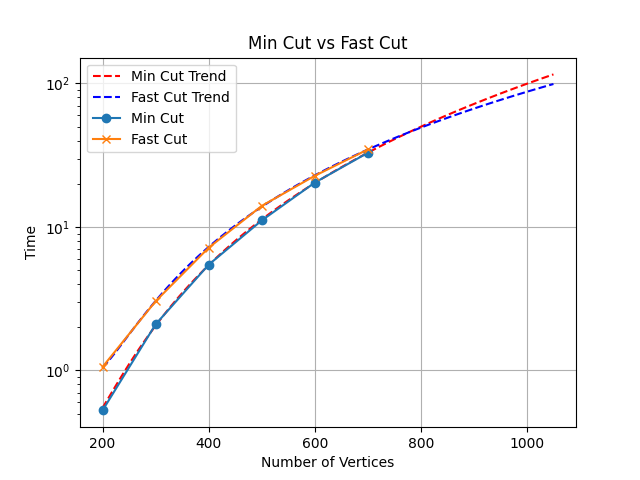
\includegraphics[width=0.7\textwidth]{../MinCut/MinCut.png}
    \caption{Execution time of Min Cut and Fast Cut \ref{alg:fastcut} algorithm}
    \label{fig:mc}
\end{figure}

\subsubsection{Results}\

We run the algorithms for 100 times for each $n$ and record the average execution time. Since our Fast Cut algorithm is a Monte Carlo algorithm, we run until getting a successful result.  The results are shown in Figure \ref{fig:mc}.

As we can see from the figure, when $n$ increases, the execution time of Fast Cut increases slower than Min Cut. When $n\approx 750$, the execution time of Fast Cut first exceeds Min Cut, which shows the advantage of Fast Cut in large-scale graphs.

\subsection{Extensions}
\subsubsection{Weighted Graph and Directed Graph}\

Weighted graph is a graph where each edge $(u,v)$ has a weight $w_{uv}$. We require the weight to be non-negative, otherwise the Min Cut problem is NP-complete since it can be reduced to Max Cut by a transformation \cite{garey1979computers}.

To handle the weighted graph, we can modify the contraction process in Algorithm \ref{alg:contract} to merge the weights of the edges.
\begin{algorithm}
    \caption{Weighted Contract}
    \label{alg:weightcontract}
    \begin{algorithmic}[1]
        \STATE \textbf{Input:} A multi-graph $G(V,E)$, a number $k$
        \STATE \textbf{Output:} A graph $G'(V',E')$
        \STATE $G'\leftarrow G$
        \WHILE{$|V'|>k$}
        \STATE randomly choose an edge $(u,v)$ from $E'$ with probability proportional to the weight of the edge
        \STATE merge $u$ and $v$ into a new vertex $w$, the weight of the edge between $w$ and $x$ is the sum of the weights of the edges between $u$ and $x$ and $v$ and $x$
        \STATE remove all self-loops
        \ENDWHILE
        \RETURN $G'$
    \end{algorithmic}
\end{algorithm}

Using the Weighted Contract algorithm, the edge with larger weight has a higher probability of being chosen. Using a similar analysis, we know Lemma \ref{lemma:9}, \ref{lemma:cut} and \ref{lemma:contract} still hold, and Lemma \ref{lemma:degree} can be modified to the weighted version.

\begin{lemma}
    In an $n$-vertex weighted graph $G$ with min-cut value $k$, no vertex has outgoing weight smaller than $k$. The total weight of the edges is at least $nk/2$.
\end{lemma}

Based on the above lemmas, we still have Theorem \ref{theorem:contract}, thus the Weighted Fast Cut algorithm can be implemented similarly.

The adjacency matrix of directed graph is not symmetric, so the Min Cut problem is different from the undirected graph.

The cost of cut $(S,V\backslash S)$ in directed graph is also defined as
\begin{align*}
    \text{cost}(S,V\backslash S)=\sum_{i\in S, j\in V\backslash S}A_{ij}
\end{align*}

Introduced by J.C. Picard and H.D. Ratliff\cite{picard1975minimum}, the weighted graph can be transformed into an equivalent undirected graph. The Min Cut problem in directed graph can be solved by solving the Min Cut problem in the equivalent undirected graph applying the Fast Cut \ref{alg:fastcut}.

\subsubsection{Improvement using data structure?}\

By using union-find data structure, we can improve the time complexity of Algorithm \ref{alg:contract}. In each iteration, we randomly select an edge and merge the two supernodes on the edge in amortized time $O(\alpha(n))$ where $\alpha(n)$ is the inverse Ackermann function. 

Since there are $m$ edges,  there are at most $m$ merging operations. Instead of randomly selecting each edge using $O(n)$ time, we generate a random permutation of the edges in $O(m)$ time, then merge the supernodes in the order of permutation. The total time complexity of the contraction process is amortized $O(m\alpha(n))$ using union find data structure. Using the naive contraction process, we can reduce the time complexity of contraction process from $O(n^2)$ to $O(m\alpha(n))$, which is more efficient for sparse graphs. However, does it really improve the time complexity of the Fast Cut algorithm like claimed in some notes\cite{CS161Lecture16} ?

Next, we analyze the time complexity of the Fast Cut algorithm for sparse graphs using union-find data structure.

% We modify the Fast Cut algorithm to the following:

% \begin{algorithm}
%     \caption{Modified Fast Cut}
%     \label{alg:modifyfastcut}
%     \begin{algorithmic}[1]
%         \STATE \textbf{Input:} A multi-graph $G(V,E)$
%         \STATE \textbf{Output:} A cut $(S,V\backslash S)$
%         \STATE $n\leftarrow |V|$
%         \IF{$n\leq 6$} 
%         \STATE compute the min-cut by brute force
%         \RETURN min-cut $(S,V\backslash S)$
%         \ELSE
%         \STATE \textcolor{red}{$t\leftarrow \lceil 1+n/2\rceil$}
%         \STATE Using Algorithm \ref{alg:contract}, perform 2 independent contraction processes to obtain graphs $H_1,H_2$ each with $t$ vertices
%         \STATE Recursively run Fast Cut on $H_1$ and $H_2$ to get cuts $(S_1,V_1\backslash S_1)$ and $(S_2,V_2\backslash S_2)$
%         \RETURN the cut with the smaller cost
%         \ENDIF
%         % \ELSE $k\leftarrow $
%     \end{algorithmic}
% \end{algorithm}

For a graph of $n$ vertices and $m$ edges, the recurrence for the running time $T(n,m)$ of Algorithm \ref{alg:fastcut} is
\begin{align*}
    T(n,m)=2T\left(\lceil 1+\frac{n}{\sqrt{2}}\rceil,m'\right)+O(\min\{m,n^2\}\alpha(n))
\end{align*}

During contraction process, the number of edges won't increase, after $k=\lceil \log_2\frac{n^2}{m}\rceil$ rounds, the number of vertices will be reduced to $n'=\frac{n}{\sqrt{2}^k}\leq \sqrt{m}$, hence
\begin{align*}
    T(n,m)&\leq 2T\left(\lceil 1+\frac{n}{\sqrt{2}}\rceil,m\right)+O(\min\{m,n^2\}\alpha(n))\\
    &\leq 2^{k}T(\sqrt{m}, m)+\sum_{i=0}^{k} 2^{i}O(\min\{m,\frac{n^2}{2^i}\}\alpha(\frac{n^2}{\sqrt{2}^i}))\\
    &\leq\frac{2n^2}{m}T(\sqrt{m},m)+O(n^2\alpha(n))\\
    &\leq \frac{2n^2}{m}m\log m+O(n^2\alpha(n))=O(n^2\log n)
\end{align*}

The success probability of the algorithm is still $\Omega(\frac{1}{\log n})$, thus the modified Fast Cut algorithm runs in $O(n^2\log n)$ time with a failure probability of $\Omega(\frac{1}{\log n})$, which is the same as the original Fast Cut algorithm. The main reason is that during contraction process, a sparse graph with $O(n)$ edges will become more and more dense, until almost complete, which is a bottleneck.

\subsection{A \texorpdfstring{$\Theta((\log n)^2)$}{ } Speedup}\

Based on Algorithm, Karger speeds up the algorithm by a factor of $\Theta((\log n)^2)$ using a quite simple algorithm \cite{karger2000minimum}, relying only on finding least common ancestors and evaluating expression-trees, and may
therefore outperform the Fast Cut algorithm in practice. In a large class of graph, it runs in $O(m)$ time. Due to the space limitation, we won't go into details of the algorithm, but give a brief introduction to introduce the main idea.

At its core is following definition:

\begin{definition}
    Let $T$ be a spanning tree of $G$. We say that a cut in $G$ $k$-respects $T$ if it cuts at most $k$ edges of $T$. We also say that $T$ $k$-constrains the cut in $G$.
\end{definition}

and 

\begin{definition}
    A cut in $G$ is $\alpha$-minimum if its value is at most
    $\alpha$ times the minimum cut value.
\end{definition}

In an unweighted $n$-vertex cycle, any set of at most $\lceil 2\alpha\rceil$ edges forms an $\alpha$-minimum cut. Therefore, the number of $\alpha$-minimum cuts can be as large as
\begin{align*}
    \binom{n}{2}+\binom{n}{4}+\cdots+\binom{n}{\lceil 2\alpha\rceil}\leq \Theta(n^{\lceil 2\alpha\rceil})
\end{align*}

and we can give an upper bound on the number of $\alpha$-minimum cuts

\begin{lemma}
    The number of $\alpha$-minimum cuts is at most
  \[
  \frac{1}{\lfloor 2\alpha \rfloor + 1 -2\alpha} \binom{n}{\lfloor
      2\alpha \rfloor}(1+O(1/n)).
  \]
\end{lemma} 

Our main idea is proving that in any graph, we can find a small set of trees such that the minimum cut 2-respects some of them. Therefore, we can find the minimum cut by enumerating only the cuts that 2-respect these few trees, which is the following theorem:

\begin{theorem}
    \label{theorem:2respect}
    Given any weighted undirected graph $G$, in $O(m+n\log^3 n)$ time we can construct a set of $O(\log n)$ spanning trees such that the minimum cut $2$-respects $1/3$ of them with high probability.
\end{theorem}

\begin{proof}
    Given a graph $G$, a skeleton $H$ is constructed using the same set of vertices by including a small random sample of the graph's edges. In Karger's previous paper\cite{karger1994random}, it's shown how to construct a skeleton graph $H$ in linear time for any $\epsilon$ such that
    \begin{itemize}
    \item $H$ has $m' = O(n\epsilon^{-2}\log n)$ edges,
    \item the minimum cut of $H$ is $c' = O(\epsilon^{-2}\log n)$,
    \item the minimum cut in $G$ corresponds (under the same vertex
      partition) to a $(1+\epsilon)$-times minimum cut of $H$.
    \end{itemize}
    Set $\epsilon=1/6$ in the skeleton construction.  Since $H$ has
    minimum cut $c'$, Gabow's algorithm\cite{gabow1991faster} can be used to find a packing in $H$ of weight $c'/2$ in $O(m'c'\log n)=O(n\log^3 n)$ time.  The original minimum cut of $G$ has at most $(1 +\epsilon)c'$ edges in $H$, so a fraction $\frac12(1-2\epsilon)=1/3$ of the trees $2$-constrain this cut in $H$.  But this $(1+\epsilon)$-minimum cut of $H$ has the same vertex partition as the minimum cut of $G$, implying that the same trees $2$-constrain the minimum cut of $G$.
\end{proof}

The following lemma is a direct consequence of the above theorem:
\begin{lemma}
    \label{lemma:2respect}
    Suppose the minimum cut that 2-respects a given tree can be found in $T(m,n)$ time.  Then the minimum cut of a graph can be found with constant probability in $T(m,n)+O(m+n\log^3 n)$ time and with high probability in $O(T(m,n)\log n+m+n\log^3 n)$ time.
\end{lemma}

Now we are left the following question: given a tree, find the minimum cut that 2-respects it. Applying the solution to the $O(\log n)$ trees gives a high probability to find the minimum cut. To introduce our approach to analyzing a particular tree, we consider a simple special case: a tree that 1-constrains the minimum cut. In other words, there is one tree edge such that, if we remove it, the two resulting connected subtrees correspond to the two sides of the minimum cut. We prove the following:

\begin{lemma}
    The minimum cut that $1$-respects a given spanning tree can be found in $O(m+n)$ time.
\end{lemma}

\begin{proof}
    Denote $\descendants{v}$ as the set of vertices that are descendants of $v$ in the rooted tree, including $v$, and $\ancestors{v}$ as the set of ancestors of $v$, including $v$. Note that $\descendants{v}\cap\ancestors{v}=\{v\}$, and $\descendants{v}\cup\ancestors{v}=V$.

    Define $\crossweight{X}{Y}$ is the total weight of edges crossing from vertex set $X$ to vertex set $Y$, $\cutval{S}$ is the value of the cut whose one side is vertex set $S$, i.e. $\crossweight{S}{\overline{S}}.$

    As a first step, suppose the tree is in fact a path $v_1,\ldots,v_n$ rooted at $v_1$.  We compute all values $\cutval{\descendants{v_i}}$ in linear time using DP. First compute $\crossweight{v_i}{\ancestors{v}_i}$ and $\crossweight{v_i}{\descendants{v}_i}$ for each $v_i$; this takes one $O(m)$-time traversal of the vertices' adjacency lists. The following recurrence applies to the cut values establishes obviously:
    \begin{align*}
    \cutval{\descendants{v_n}} &= \crossweight{v_n}{\ancestors{v}_n}\\ 
    \cutval{\descendants{v_i}} &= \cutval{\descendants{v}_{i+1}}+\crossweight{v_i}{\ancestors{v}_i} -\crossweight{v_i}{\descendants{v}_i}
    \end{align*}

    It takes $O(n)$ time to compute all $n$ cut values. We know extend our DP function from paths to general trees. For any function $f$, we define treefix sum of $f$, denoted $\descendants{f}$, as
    \begin{align*}
        \descendants{f}(v)=\sum_{w\in\descendants{v}}f(w)
    \end{align*}

    Then define $\delta(v)$ as the weighted degree of $v$, $\rho(v)$ as the total weight of edges whose endpoints' least common ancestor is $v$. $\descendants{\delta}(v)$ counts all edges that leaving descendants of $v$, this not only counts each edge crossing the cut defined by $\descendants{v}$, but also doubly count all edges with both endpoints descended from $v$, which happens if and only if its least common ancestor is in $\descendants{v}$. Hence, we have the following lemma:

    \begin{lemma}
        \label{lemma:delta}
        \begin{align*}
            \cutval{\descendants{v}} = \descendants{\delta}(v)-2\descendants{\rho}(v)
        \end{align*}
    \end{lemma}

    Computing $\delta(v)$ for all $v$ in $O(m)$ time is trivial. Note that least common ancestors of each edge can be found in $O(m)$ time\cite{gabow1983linear}, hence $\rho(v)$ can be also computed in linear time, so does $\descendants{\delta}(v)$ and $\descendants{\rho}(v)$. From these quantities, using Lemma \ref{lemma:delta}, all $\cutval{\descendants{v}}$ can be determined in $O(m+n)$ time, which completes the proof.
\end{proof}

Using the similar idea, we can prove the following lemma:

\begin{lemma}
    \label{lemma:respect}
    The values of all cuts that $2$-respect a given tree can be found in $O(n^2)$ time.
\end{lemma}

\begin{proof}
    We say two vertices are incomparable, e.g. $v\perp w$ if $v \notin \descendants{w}$ and $w \notin \descendants{v}$.  In other words, $v$ and $w$ incomparable if and only if they are not on the same root-leaf path. Suppose the minimum cut that 2-respects the tree cuts vertices $v$ and $w$ with their parents. If $v\perp w$, parent edges of $v$ and $w$ define a cut with value
    \begin{align*}
        \cutval{\descendants{v}\cup\descendants{w}} =\cutval{\descendants{v}}+\cutval{\descendants{w}} -2\crossweight{\descendants{v}}{\descendants{w}} 
    \end{align*}
    Otherwise, w.l.o.g $v \in \descendants{w}$, then their parent edges define a cut with value
    \begin{align*}
        \cutval{\descendants{w}-\descendants{v}}&=\cutval{\descendants{w}}-\cutval{\descendants{v}}+2\crossweight{\descendants{v}}{\descendants{w}-\descendants{v}}\\
        &=\cutval{\descendants{w}}-\cutval{\descendants{v}}+2\crossweight{\descendants{v}}{\descendants{w}}-4\descendants{\rho}(v)
    \end{align*}
    
    We already show how to compute all $\cutval{\descendants{v}}$ and $\descendants{\rho}(v)$ in $O(m)$-time, similarly $\crossweight{\descendants{v}}{\descendants{w}}$ can be computed using treefix sum of $f_v(w)=\crossweight{v}{w}$ (which is the weight of edge $(v,w)$), then for each $v,w$, all $n^2$ values
    \begin{align*}
        g_w(v)=\descendants{f_v}(w)=\sum_{u\in\descendants{w}}\crossweight{v}{u}=\crossweight{v}{\descendants{w}}
    \end{align*}
    can be computed in $O(n^2)$ time, as well as
    \begin{align*}
        \descendants{g_w}(v)=\sum_{u\in\descendants{w}}\crossweight{v}{u}=\crossweight{\descendants{v}}{\descendants{w}}
    \end{align*}
    after having all $\descendants{g_w}(v)$, computing values of all cuts that $2$-respect the tree is trivial, which completes the proof.
\end{proof}

Combine Lemma \ref{lemma:respect} with Lemma \ref{lemma:2respect}, we know the minimum cut of graph can be found with constant probability($\sim 1/3$) in $O(n^2)$-time, and with high probability in $O(n^2\log n)$ time, which implements a $\Theta((\log n)^2)$ speedup. More generally, we can prove the following theorem:
\begin{theorem}
    Given any weighted undirected graph $G$, the minimum cut can be found in $O(cn^2\log n)$ time with a failure probability of $O(1/n^c)$ using a Monte Carlo algorithm.
\end{theorem}

% \subsection{Advanced Algorithm}

% In recent years, there have been several advancements in the algorithms for the Min Cut problem. One notable approach is the use of spectral techniques and semidefinite programming (SDP). These methods leverage the properties of the graph's Laplacian matrix and eigenvalues to find approximate solutions to the Min Cut problem.

% \paragraph{Spectral Methods}

% Spectral methods involve the use of the graph Laplacian matrix, which is defined as $L = D - A$, where $D$ is the degree matrix and $A$ is the adjacency matrix. The eigenvalues and eigenvectors of the Laplacian matrix provide valuable information about the graph's structure. The second smallest eigenvalue, known as the Fiedler value, and its corresponding eigenvector, the Fiedler vector, can be used to partition the graph into two sets, providing an approximation to the Min Cut.

% \paragraph{Semidefinite Programming}

% Semidefinite programming (SDP) is a powerful optimization technique that can be used to approximate the Min Cut problem. The Goemans-Williamson algorithm is a well-known SDP-based approximation algorithm for the Max Cut problem, which can be adapted for the Min Cut problem. The algorithm involves solving an SDP relaxation of the Min Cut problem and then using a randomized rounding technique to obtain a cut.

% \begin{algorithm}
% \caption{Goemans-Williamson Algorithm for Min Cut}
% \label{alg:goemans-williamson}
% \begin{algorithmic}[1]
%     \STATE \textbf{Input:} Graph $G=(V,E)$ with adjacency matrix $A$
%     \STATE \textbf{Output:} Approximate Min Cut $(S, V \setminus S)$
%     \STATE Solve the SDP relaxation of the Min Cut problem to obtain a matrix $X$
%     \STATE Perform Cholesky decomposition on $X$ to obtain a matrix $L$
%     \STATE Randomly choose a vector $r$ from a Gaussian distribution
%     \STATE Compute the cut $(S, V \setminus S)$ by partitioning the vertices based on the sign of the dot product of their corresponding rows in $L$ with $r$
%     \RETURN $(S, V \setminus S)$
% \end{algorithmic}
% \end{algorithm}

% These advanced algorithms provide approximate solutions to the Min Cut problem with provable guarantees on the quality of the solution. While they may not always find the exact Min Cut, they are often much faster than exact algorithms, especially for large graphs.

\subsection{Open Problems}\

Despite the significant progress in algorithms for the Min Cut problem, several open problems remain. We highlight key challenges and directions for future research:
\begin{enumerate}
    \item \textbf{Improved Approximation Algorithms:} Develop faster algorithms with better approximation guarantees, especially for graphs with specific structures or properties
    \item \textbf{Dynamic Graphs:} Extend these algorithms to handle dynamic graphs, where the graph structure changes over time
    \item \textbf{Parallel and Distributed Algorithms:} Finding efficient parallel and distributed algorithms for the Min Cut problem is an important area of research, especially given the increasing size of real-world graphs
    \item \textbf{Generalizations and Variants:} Explore generalizations and variants of the Min Cut problem, such as weighted graphs, directed graphs, and multi-way cuts
\end{enumerate}

By addressing these problems, researchers can further advance the state of the art in algorithms for the Min Cut problem.

\section{Other Related Problems}

\subsection{Minimum Spanning Tree (MST)}

\subsubsection{Introduction}\

The Minimum Spanning Tree (MST) problem is another classic problem in graph theory that involves finding a spanning tree of minimum weight in a connected, undirected graph. The problem is defined as follows:

\begin{definition}
    Given an undirected graph $G=(V,E)$ with edge weights $w:E\to \mathbb{R}$, the Minimum Spanning Tree problem is to find a spanning tree $T$ of $G$ that minimizes the sum of the edge weights in $T$.
\end{definition}

The MST problem has many practical applications, such as in network design, clustering, and optimization. Several algorithms have been developed to solve the MST problem efficiently, including Prim's algorithm, Kruskal's algorithm, and Boruvka's algorithm. A famous open problem is how to solve MST in linear time. In this section, we will introduce a Linear Time Randomized Algorithm for MST.

\subsubsection{Boruvka's Algorithm}\

Let's start with a particular greedy strategy for the MST problem, known as Boruvka's algorithm. The algorithm works as follows:
\newline
\begin{algorithm}
\caption{Boruvka's Algorithm for MST}
\label{alg:boruvka}
\begin{algorithmic}[1]
    \STATE \textbf{Input:} Graph $G=(V,E)$ with edge weights $w:E\to \mathbb{R}$
    \STATE \textbf{Output:} Minimum Spanning Tree $T$
    \STATE Initialize $T$ to be an empty set
    \WHILE{$T$ is not a spanning tree}
        \STATE For each connected component $C$ of $T$, find the minimum-weight edge $e$ with exactly one endpoint in $C$
        \STATE Add $e$ to $T$
    \ENDWHILE
    \RETURN $T$
\end{algorithmic}
\end{algorithm}

Boruvka's algorithm is a simple and efficient algorithm for finding the MST of a graph. It works by iteratively adding the minimum-weight edge that connects two connected components of the current spanning tree. The algorithm terminates when the spanning tree is fully connected, i.e., when there is only one connected component. The key observation here is MST for $G$ must contain the edge $(v,w)$ which is the minimum-weight edge incident on $v$.

Boruvka's algorithm reduces MST problem in an $n$-vertex graph with $m$ edges to MST problem in a graph with at most $\frac{n}{2}$ vertices and $m$ edges in $O(m+n)$-time. The worst-case time complexity is $O(m\log n)$.

\subsubsection{Light and Heavy Edges}\

Before introducing the Linear Time Randomized Algorithm for MST, we first introduce concepts called \textit{light edge} and \textit{heavy edge}.

\begin{definition}
    Given a graph $G=(V,E)$ with edge weights $w:E\to \mathbb{R}$, fix a forest $F$ of $G$. $w_F(u,v)$ is the maximum weight of an edge on the path from $u$ to $v$ in $F$ if exists, and set to be $\infty$ when $u$ and $v$ are disconnected in $F$. An edge $e\in E$ is said to be $F$-\textit{heavy} if $w(u,v)>w_F(u,v)$. Otherwise, it is $F$-\textit{light}.
\end{definition}

It's easy to check all edges in $F$ are $F$-light. The following lemma is a direct consequence of the definition:

\begin{lemma}
    Let $F$ be any forest in the graph $G$. If an edge $(u,v)$ is $F$-heavy, then it is not in the MST of $G$.
\end{lemma}

The idea to define light and heavy edges is to improve a forest $F$. Specifically, adding an edge $e$ to $F$ will reduce the number of connected components in $F$, or generate a cycle in $F$ such that we can remove the edge of the largest weight in the cycle. An $F$-light edge is a candidate to be added to $F$ to improve it, while an $F$-heavy edge is not. Based on this observation, a tree $T$ is a MST if and only if it is a forest such that all $T$-light edges are in $T$. So we can verify whether a tree is a MST by checking whether all its edges are light. In fact, the following theorem holds:

\begin{theorem}
    \label{theorem:heavy}
    Given a graph $G$ and a forest $F$, all $F$-heavy edges in $G$ can be identified in $O(m+n)$ time.
\end{theorem}
\begin{proof}
    First, we preprocess the forest $F$ to answer Least Common Ancestor (LCA) queries efficiently. This can be done using techniques like Binary Lifting or Euler Tour with RMQ, both of which take $O(n)$ time for preprocessing and $O(1)$ time per query\cite{bender2000lca}. After building the LCA data structure, using the algorithm proposed by Tarjan\cite{doi:10.1137/0221070} to compute the maximum edge weight on the path between any two vertices in $F$ in $O(n+m)$ time. The overall time complexity is $O(n + m)$ for identifying all $F$-heavy edges given the forest $F$.
\end{proof}

\subsubsection{Linear Time Randomized Algorithm for MST}\

Based on the algorithm above, we can use random sampling to identify and eliminate heavy edges in MST. Consider a random graph $G(p)$ obtained by independently including each edge of $G$ in $G(p)$ with probability $p$. The connectivity of $G(p)$ is not guaranteed. The linear time randomized algorithm for MST is based on the following lemma:

\begin{lemma}
    \label{lemma:randomizedmst}
    Let $F$ be the minimum spanning forest in the random graph $G(p)$. Then the number of $F$-light edges in $G$ is stochastically dominated by a random variable $X$ that has negative binomial distribution with parameters $n$ and $p$. In particular, the expected number of $F$-light edges in $G$ is at most $\frac{n}{p}$.
\end{lemma}
\begin{proof}
    Consider following process: sort edges of $G$ in the order of increasing weight, construct $G(p)$ by including each edge in this order with probability $p$. The minimum spanning forest of $G(p)$ can be constructed during the process. The edge is added to $F$ if and only if the two endpoints $u$ and $v$ belong to different connected components of $F$. The observations are:
    \begin{enumerate}
        \item edges are never removed from $F$ during this process.
        \item the $F$-lightness of $e_i$ only depends on the connected components of $F$ after $e_i$ is added to $F$.
        \item the edge $e_i$ is $F$-light finally if and only if it's $F$-light when it's added to $F$.
    \end{enumerate}
    Define phase $k$ as starting after forest $F$ has $k-1$ edges and end when $F$ has $k$ edges. The number of $F$-light edges considered during this phase has geometric distribution with parameter $p$. Suppose $F$ grows in size from 0 to $s$. The number of $F$-light edges considered during this process is sum of $s$ independent geometric random variables with parameter $p$.

    To compute the $F$-light edges processed after but not chosen in $G(p)$, we can continue flipping coins until we have $n$ successes. The number of failures before the $n$-th success is a negative binomial random variable with parameters $n$ and $p$\footnote{The negative binomial distribution is the distribution of the number of failures before the $n$-th success in a sequence of independent Bernoulli trials.}. 

    Since $s$ is at most $n-1$, the number of $F$-light edges is stochastically dominated by a negative binomial distribution with parameters $n$ and $p$. The expected number of $F$-light edges is at most $\frac{n}{p}$.
\end{proof}

Based on this, we propose the following Linear Time Randomized Algorithm for MST\cite{karger1995randomized}:

\begin{algorithm}
    \caption{Linear Time Randomized Algorithm for MST}
    \begin{algorithmic}[1]
    \label{alg:randomizedmst}
    \STATE \textbf{Input:} Undirected Weighted Graph $G=(V,E)$ with edge weights $w:E\to \mathbb{R}$
    \STATE \textbf{Output:} Minimum Spanning Tree $T$
    \STATE Using three applications of Boruvka's phases interleaved with simplification of the contracted graphs, compute a graph $G_1$ with at most $\frac{n}{8}$ vertices and let $C$ be the set of edges contracted during the three phases. If $G$ is empty then exit and return $F=C$.
    \STATE Let $p=\frac{1}{2}$ and let $G_2=G_1(p)$ be a randomly sampled subgraph of $G_1$.
    \STATE Recursively applying algorithm MST, compute the minimum spanning forest $F_2$ of $G_2$.
    \STATE Using a linear-time verification algorithm, identify the $F_2$-heavy edges in $G_1$, delete them to obtain a graph $G_3$.
    \STATE Recursively applying algorithm MST, compute the minimum spanning forest $F_3$ for graph $G_3$.
    \RETURN $C\cup F_3$
    \end{algorithmic}
\end{algorithm}

Since all $F_2$-heavy edges are impossible to be included in the MST by Theorem \ref{theorem:heavy}, we can safely remove them from $G_1$ to obtain $G_3$. The correctness of the algorithm is based on this. The time complexity of the algorithm is guaranteed by the following theorem:

\begin{theorem}
    The expected running time of Algorithm \ref{alg:randomizedmst} is $O(m+n)$.
\end{theorem}
\begin{proof}
    Define $T(n,m)$ as the expected running time of Algorithm \ref{alg:randomizedmst} on graphs with $n$ vertices and $m$ edges. Boruvka's algorithm takes $O(m+n)$ time, and produce a graph $G_1$ with at most $\frac{n}{8}$ vertices and $m$ edges. Random sampling to produce $G_2=G_1(\frac{1}{2})$ with $\frac{n}{8}$ vertices and an expected number of edges equal to $\frac{m}{2}$, which takes $O(m+n)$ time. Finding the minimum spanning forest $G_2$ has expected cost $T(\frac{n}{8},\frac{m}{2})$, by induction and linearity of expectation.

    The verification to identify $F_2$-heavy edges in $G_1$ takes $O(m+n)$ time using \ref{theorem:heavy}. By Lemma \ref{lemma:randomizedmst}, the expected number of $F_2$-light edges in $G_1$ is at most $\frac{n}{4}$. Finding the MST of $G_3$ has expected cost $T(\frac{n}{8},\frac{n}{4})$, return the union of $C$ and the MST of $G_3$ takes $O(m+n)$ time. Putting all together, we have
    \begin{align*}
        T\left(n,m\right)\leq T\left(\frac{n}{8},\frac{m}{2}\right)+T\left(\frac{n}{8},\frac{n}{4}\right)+c\left(m+n\right)
    \end{align*}
    for some constant $c$. The solution to this recurrence is $O(m+n)$, hence the expected running time of Algorithm \ref{alg:randomizedmst} is $O(m+n)$.
\end{proof}

\subsubsection{Open Problems}\

Despite significant advancements in algorithms for the Minimum Spanning Tree problem, several open problems remain:

\begin{enumerate}
    \item \textbf{Linear Time Deterministic MST Algorithms:} While randomized algorithms, like Karger's, achieve near-linear time complexity, it is still an open question whether a deterministic linear-time algorithm exists for finding the MST in undirected, weighted graphs. Achieving this would be a major breakthrough, especially in deterministic graph processing.
    \item \textbf{MST in Hypergraphs:} Extending the MST problem to hypergraphs, where edges can connect more than two vertices, is less understood and lacks efficient algorithms. The MST definition in hypergraphs is not as straightforward as in regular graphs, and finding optimal algorithms for this generalization, including approximation methods, remains an open question.
    \item \textbf{Streaming MST:} In streaming settings, where edges are processed sequentially due to memory constraints, designing efficient algorithms to compute or approximate the MST is challenging. The open problem here is to find single-pass, memory-efficient algorithms that can construct the MST or approximate it closely with minimal space usage, especially for massive graphs.
\end{enumerate}

By addressing these open problems, researchers can further advance the SOTA in algorithms for the Minimum Spanning Tree problem and its generalizations.

\subsection{Exact Matching (EM)}

\subsubsection{Introduction}\

The Exact Matching (EM) problem on a graph is defined as follows:
\begin{definition}
    Given a graph $G=(V,E)$ with each edge $e$ having a color red or blue, and a non-negative integer $k$, the Exact Matching problem is to decide whether $G$ has a perfect matching $\mathcal{M}$ such that exactly $k$ edges in $\mathcal{M}$ are red.
\end{definition}
This problem is first proposed by Papadimitriou and Yannakakis in 1982 \cite{papadimitriou1982complexity}. EM is conjectured at first to be \textbf{NP}-complete. However, Ketan Mulmuley, Umesh V Vazirani and Vijay V Vazirani\cite{mulmuley1987matching} showed that EM is in \textbf{RP} - that is, it can be solved in polynomial time using randomized algorithms. Furthermore, EM was later shown to be in \textbf{RNC} (can solve in poly-logarithmic time, i.e. $O(\log^cn)$, using polynomial parallel processors).

In this subsection, we will discuss one of the random algorithm of EM.

\subsubsection{Pfaffian and Orientation}\

For a undirected simple graph $G$, we can define a \textbf{weighted orientation} as follows:

\begin{definition}
Suppose $D$ is a field. A mapping $\mathcal{X}:V\times V\to D$ of $G$ is a weighted orientation, if for each $(x,y)\in E(G)$, $\mathcal{X}(x,y)+\mathcal{X}(y,x)=0$; for each $(x,y)\not\in G$, $\mathcal{X}(x,y)=0$.
\end{definition}
Using this definition, we can now define the Pfaffian:

\begin{definition}
For a weighted orientation $\mathcal{X}$ of $G$, the Pfaffian of $\mathcal{X}$, $\mathbf{Pf}(\mathcal{X})$ is defined as
$$\sum\limits_{M\in \mathcal{M}} t_M.$$
Here, $\mathcal{M}$ is all perfect matchings of $G$, and $t_M$ is defined as
\begin{align}
t_M=\mathrm{sgn}(\sigma)\cdot \mathcal{X}(i_1,i_2)\mathcal{X}(i_3,i_4)\cdots \mathcal{X}(i_{2n-1},i_{2n}), \label{defpffa}
\end{align}
where $\sigma=(i_1i_2\cdots i_{2n})$ is a permutation of $V(G)$ such that $M=\{(i_{2j-1},i_{2j})\}_{1\le j\le n}$.
\end{definition}
Note that, although for a matching $M$, the representation permutation $\sigma$ is not unique, but the definition of $t_M$ is consistent. For instance, when we swap $i_1,i_2$, the sign of $\sigma$ changes, and $\mathcal{X}(i_1,i_2)=-\mathcal{X}(i_2,i_1)$, so \eqref{defpffa} remains the same; when we swap $(i_1,i_2)$ with $(i_3,i_4)$, the similar fact is also easy to verify.

\subsubsection{A Polynomial Algorithm to Calculate Pfaffian}\

To derive Pfaffian for a weighted orientation, we must assume that the arithmetic operations in $D$ is $O(1)$. We claim Lemma \ref{pffa_eq_det}, which directly leads to a polynomial algorithm to calculate Pfaffian.

\begin{definition}
For a weighted orientation $\mathcal{X}$, define \textbf{Orientation Matrix} $A_G(\mathcal{X})$ to be
$$A_G(\mathcal{X})=(\mathcal{X}_{ij})_{1\le i,j\le |V|}.$$
\end{definition}

\begin{lemma}
\label{pffa_eq_det}
For a weighted orientation $\mathcal{X}$, we have
$$\det(A_G(\mathcal{X}))=\mathbf{Pf}(\mathcal{X})^2.$$
\end{lemma}
\begin{proof}
\textit{(Sketch)} Consider each term in the expansion of $\det(A_G(\mathcal{X}))$. Each term is a product of $|V|$ elements, one from each row and column of $A_G(\mathcal{X})$. These $|V|$ elements represent $n$ oriented edges, satisfying each vertex in $V$ has exactly one outward degree and inward degree. Thus, these edges form several cycles.

Suppose there have a odd cycle. Consider changing the orientation of each edges in this odd cycle, then the sign of the term in the determinant changes, but $t_M$ does not change. So these two terms cancel each other.

Therefore, we can only consider those terms that form a bipartite graph. For each term, we can color the edges into two colors, such that each color is a perfect matching. This yields a correspondence to a term in $\mathbf{Pf}(\mathcal{X})^2$. The detailed calculation of the sign is omitted.
\end{proof}
Since we can use Gaussian elimination to calculate the determinant of a matrix in $O(n^3)$ time (where $n=|V|$), we can use this lemma to calculate the Pfaffian in $O(n^3)$ time.

\subsubsection{Randomized Algorithm for EM}\

Now, assume $D=\mathbb{R}(x)$, where $x$ is an indeterminate. We define a weighted orientation $\mathcal{X}$ as follows: for every red edge $e=(a,b)$, let $\mathcal{X}(a,b)=f(a,b)x$; for every blue edge, let $\mathcal{X}(a,b)=f(a,b)$. Here, $f(a,b)\in \mathbb{R}$. 

We can easily see that $\mathbf{Pf}(\mathcal{X})$ is a polynomial in $x$. Most importantly, the $x^k$ coefficient of $\mathbf{Pf}(\mathcal{X})$ represents all the perfect matchings with exactly $k$ red edges. Furthermore, if $f$ is randomly chosen from $\mathbb{R}$, then this coefficient is likely to be non-zero if it is non-zero initially.

However, to give a specific bound of the probability of success, we can let $D=\mathbb{F}_p(x)$, and $f(a,b)\in \mathbb{F}_p$, where $p$ is a sufficiently large prime. 

Thus, the algorithm is as follows: we randomly choose $f(a,b)\in \mathbb{F}_p$ for all edges, and calculate the Pfaffian of $\mathcal{X}$. If the $x^k$ coefficient is non-zero, then we output ``YES''; otherwise, we do this process again. If the number of trials exceeds a certain threshold $N$, we output ``NO''.

This algorithm guarantees to run in polynomial time iff $N=O(\text{poly}(n))$.

\subsubsection{Correctness: Schwarz's Lemma}\

Note that if we see $f(a,b)$ as an individual indeterminate, the $x^k$ coefficient of Pffafian is a polynomial in all $f(a,b)$. When all indeterminate $f(a,b)$ are randomly chosen, we will bound the probability of success by Schwartz–Zippel Lemma \cite{10.1145/322217.322225}.

\begin{lemma}
\label{schwarz}
Let $x_1,x_2,\cdots,x_n$ be $n$ indeterminates, and $P\in \mathbb{F}_p(x_1,x_2,\cdots,x_n)$ is a non-zero polynomial of degree $\le d$. Then,
$$\#\{(x_1,x_2,\cdots,x_n)\in \mathbb{F}_p^n:P(x_1,\cdots,x_n)=0\}\le p^n\cdot \dfrac{d}{p}.$$
\end{lemma}

Obviously, the $x^k$ coefficient of Pfaffian is a polynomial of degree $\le n$ in all $f(a,b)$. So, if we select $p>2n$, then the probability of success is at least $\dfrac{1}{2}$, proving that \textbf{EM} $\in$ \textbf{RP}.

\subsubsection{Open Problems}\

There are several open problems related to the Exact Matching problem: 
\begin{enumerate}
    \item \textbf{Deciding whether EM is in P} has remained an open problem for almost four decades and little progress has been made even for very restricted classes of graphs;
    \item \textbf{Derandomizing} matching problems from the algorithm in \textbf{RNC} class \cite{svensson2017matching}.
    \item \textbf{EM} together with other related problems, such as \textbf{TkPM}, remains open to design a better \textbf{deterministic approximation algorithm}.
\end{enumerate}

\section{Our Proposed Problem: Optimal Point Traversing Path}

\subsection{Problem Definition}\

Given a graph $G(V,E)$, and a set of points $P\subseteq V$, called \textbf{key points}, the \texttt{Minimum Point Traversing Path} problem is to find a path that traverses all points in $P$ \textbf{at least once}, such that the length of the path (number of edges) is minimized. 

In fact, \texttt{MPTP} is NP-complete. We can prove \texttt{Hamiltonian-Path} $\le_P$ \texttt{MPTP} by setting $P=V$.

An easier version of the problem is \texttt{Optimal Point Traversing Path (OPTP)}. For every $P'\subseteq V$, let $\xi(P')$ be minimum length of path that traverses all points in $P'$ at least once. For $1\le i\le n$, let
$$\xi(i) = \max\limits_{|P'|=i} \xi(P').$$
For an algorithm $\mathcal{A}$, given $G,P$, it can output a path of length $\mathcal{A}_P$. Let
$$\xi_A(i) = \max\limits_{|P'|=i} \mathcal{A}_{P'}.$$
The \texttt{OPTP} problem requires to find an algorithm $\mathcal{A}$, such that
$$\lim\limits_{|V|\to \infty} \dfrac{\xi_A(f(|V|))}{\xi(f(|V|))}=1.$$
$f$ is an arbitrary non-decreasing function. In the following discussion, we assume $f(x)=\lceil\sqrt{x}\rceil$. Note that the choice of $f$ does not affect the difficulty of the problem - when $|V|$ increases but $i$ stays the same, the problem becomes strictly harder.

The intuition is, for a large graph, given a set of key points $P$, we can always find a path traversing all points in $P$ with a reasonable length, which means it is not longer than the optimal solution in the worst case. 

In real life scenarios, the key points may represent the user's location. The edges are the roads. Imagine a courier want to deliver packages to all the users, he needs to traverse these points at least once. In order to handle the worst serving efficiency, one need to minimize the maximum possible length, which is lower bounded by the optimal solution in the worst case. So, \texttt{OPTP} is a reasonable model for real life applications.

\subsection{A Sublinear Algorithm On a Special Case: Grid Graph}\

Since we model the key points to be the user's location, and the graph to be the road, one may consider the graph to be a \textbf{grid graph}. Formally, given a positive integer $n$, a grid graph is a graph $G_n$ with $n^2$ vertices, which are arranged in an $n\times n$ grid. Each vertex is connected to its adjacent vertices in the grid, i.e. the vertex $(i,j)$ is connected to $(i\pm 1,j)$ and $(i,j\pm 1)$.

With the supposition above, we can assume the key point set $|P|=n$, which is a sensible assumption.

\subsubsection{The Lower Bound of \texorpdfstring{$\xi$}{ }}\

Now consider the worst case $\xi(n)$. 

\begin{lemma}
\label{hahaha1}
For every positive integer $n$, we have $\xi(n+1)\ge \sqrt{2}n^{3/2}-10n$.
\end{lemma}
\begin{proof}
Let the grid
$$V(G_{n+1})=\{(i,j):0\le i,j\le n,\ i,j\in \mathbb{Z}\}.$$
For any point $X\in [0,n]^2$, let $f(X)$ be the point $v\in V$ that is the closest to $X$ (w.r.t. Manhattan distance: $d(\mathbf{x},\mathbf{y})=|x_1-x_2|+|y_1-y_2|$).\\
Let $M=\lfloor \sqrt\frac{n}{2}\rfloor$. Let
$$S=\left\{\left(\dfrac{s\sqrt{n}}{\sqrt{2}},\dfrac{t\sqrt{n}}{\sqrt{2}}\right):s,t\in \mathbb{N},\ s+t\equiv 1\pmod 2,\ s,t\le 2M\right\}.$$
Since $\sqrt{2}M\le \sqrt{n}$, we have
$$\dfrac{s\sqrt{n}}{\sqrt{2}},\dfrac{t\sqrt{n}}{\sqrt{2}}\le \sqrt{2}M\sqrt{n}\le n,$$
which means $S\subseteq [0,n]^2$. Furthermore,
$$|S|=2M^2\le 2\cdot \left(\sqrt{\dfrac{n}{2}}\right)^2=n,$$
and
$$|S|=2M^2\ge 2\cdot \left(\sqrt{\dfrac{n}{2}}-1\right)^2\ge n-4\sqrt{n}+1.$$
Obviously, for any $A,B\in S$, we have $d(A,B)\ge \sqrt{2n}$. Thus, for every $X\in S$, we add $f(X)$ into $P$. Since $|S|\le n$, we have $|P|\le n$ (Note that a smaller $|P|$ means a smaller answer). Since for every $X\in [0,n]^2$, $d(X,f(X))\le 1$, we have
$$d(X,Y)\ge \sqrt{2n}-2,\quad \forall X,Y\in P.$$
Thus, the minimal length of the traversing path is at least
$$(\sqrt{2n}-2)(|S|-1)\ge (\sqrt{2n}-2)(n-4\sqrt{n})\ge \sqrt{2}\cdot n^{3/2}-10n.$$
\end{proof}

\subsubsection{The Randomized Algorithm}\

Now we give an algorithm $A$, that runs in $o(n^2)=o(|V|)$ time (i.e. \textbf{sublinear}), to solve \texttt{OPTP} on $G_{n+1}$. Using Lemma \ref{hahaha1}, we only need to show that $A$ outputs a path of length at most $\sqrt{2}n^{3/2}+10n$ in every case.

\begin{definition}
    \label{def5.1}
A process of \textbf{traversing $[l,r)$ from left to right} is to visit all vertices in $P\cap ([l,r)\times [0,n])$ by the increasing order of $x$-coordinate. Specifically: suppose $P\cap ([l,r)\times [0,n))=\{v_1,v_2,\ldots,v_k\}$, with
$$x_{v_1}\le x_{v_2}\le \cdots\le x_{v_k},$$
where $x_{v}(v\in V)$ is the $x$-coordinate of $v$ in the grid. We start on point $(l,0)$, and visit $v_1,v_2,\ldots,v_k$ in order, and finally reach $(r,n)$. When visiting, we always choose the shortest path to the next point.
\end{definition}

Similarly, we can define a ``reverse'' process:
\begin{definition}
A process of \textbf{traversing $[l,r)$ from right to left} is defined as: suppose $P\cap ([l,r)\times [0,n))=\{v_1,v_2,\ldots,v_k\}$ in the same order in \ref{def5.1}. We start on point $(l,n)$, visit $v_k,v_{k-1},\ldots,v_1$ in order, and finally reach $(r,0)$.
\end{definition}

Now, we want to divide $[0,n]$ into some intervals $[l_i,r_i)$, satisfying $l_i=r_{i-1}$, and perform the following process one-by-one: traversing $[l_1,r_1)$ from left to right; traversing $[l_2,r_2)$ from right to left; traversing $[l_3,r_3)$ from left to right; and so on. 

Let $T$ be an undetermined positive integer. \text{Randomly} choose $0\le b<T$ with equal probability, and set all $l_i=b+iT$ and $r_i=b+(i+1)T$ \textit{(we need $[0,b)$ for the case $b\ge 1$, and the last $r_i$ may exceed $n$. However, we can ignore this, and it does not make the answer smaller)}. This is the algorithm $A$. 

\subsubsection{Correctness Proof}\

Let $\ell_b$ be the length of the path when $A$ chooses $b$, we now prove that $\mathbb{E}_b[\ell_b]\le \sqrt{2}n^{3/2}+10n$ if $T$ is carefully chosen.

Suppose we are doing the process of traversing $[l,r)$ from left to right, and $P\cap ([l,r)\times [0,n))=\{v_1(x_1,y_1),v_2(x_2,y_2),\ldots,v_k(x_k,y_k)\}$ in the order of $x$-coordinate, i.e. $x_1\le x_2\le \cdots\le x_k$. The number of step in this process can be calculated as
\begin{align}
V_{\text{left}\to \text{right}}(l,r):=n+\left(|l-y_1|+\sum\limits_{i=1}^{k-1} |y_{i}-y_{i+1}|+|y_k-r|\right). \label{ggg}
\end{align}
The reason is as above: at $x$-coordinate, we always go in one direction, so the number of steps is $n$; at $y$-coordinate, from $v_i$ to $v_{i+1}$, we need $|y_i-y_{i+1}|$ steps, adding the contribution of $(l,0)\to v_1$ and $v_k\to (r,n)$, we get \eqref{ggg}.

\begin{definition}
\label{def5.3}
For a point $A_i$, if it lies in a strip $[l,r)$, define the \textbf{distance function} $w(A_i)=\max\{y_i-l,r-y_i\}$.
\end{definition}
We use the definition \ref{def5.3} to give a bound of \eqref{ggg}.

\begin{lemma}
    \label{ineq}
For every two points $A_i,A_{i+1}$ which are in the same strip $[l,r)$, we have
$$|y_i-y_{i+1}|\le w(v_i)+w(v_{i+1})-T,$$
where $T=|r-l|$.
\end{lemma}
\begin{proof}
W.L.O.G let $y_i\ge y_{i+1}$. Then, since $r\ge y_i\ge y_{i+1}\ge l$, we have
$$|y_i-y_{i+1}|+|r-l|=|r-y_{i+1}|+|y_i-l|\le w(v_{i+1})+w(v_i).$$
\end{proof}

Using Lemma \ref{ineq}, we have
\begin{align*}
V_{\text{left}\to \text{right}}(l,r) &= n+\left(|l-y_1|+\sum\limits_{i=1}^{k-1} |y_{i}-y_{i+1}|+|y_k-r|\right)\\
&\le n + w(v_1) + \sum\limits_{i=1}^{k-1} (w(v_i)+w(v_{i+1})-T) + w(v_k)\\
&= n + 2\sum\limits_{i=1}^{k} w(v_i) - (k-1)T\\
&= n + \sum\limits_{i=1}^k (2w(v_i)-T) + T. 
\end{align*}
Similarly, we get
$$V_{\text{right}\to \text{left}}(l,r)\le n + \sum\limits_{i=1}^k (2w(v_i)-T) + T. $$
Adding up each $[l,r)$, observe that the number of strips is at most $\frac{n}{T}+1$, we have
\begin{align*}
\#\text{steps} &= \sum\limits_{[l,r)} V(l,r)\\
&\le (n+T)\cdot \left(\dfrac{n}{T}+1\right)+\sum\limits_{i=1}^n (2w(V_i)-T),
\end{align*}
where $P=\{V_1,\cdots,V_n\}$ is the set of key points. To bound the expectation of the number of steps, we need to first bound the expectation of $w(V_i)$.

\begin{lemma}
    \label{lemma5.3}
For every $V\in P$, if $0\le b<T$ is uniformly chosen, and all strips $[l_j,r_j)$ is generated by
$$l_j=b+jT,\quad r_j=b+(j+1)T,$$
we have
$$\mathbb{E}[w(V)]\le \dfrac{3T}{4}+1.$$
\end{lemma}
\begin{proof}
There is equal probability for $y_V-l$ to be $0,1,\cdots,T-1$, and the corresponding value of $w(V)$ is
$$T,T-1,T-2,\cdots,T-2,T-1,T,$$
respectively. Thus, we have for an even $T$,
$$\mathbb{E}[w(V)]=\dfrac{1}{T}\cdot \dfrac{1}{4}(T+1)(3T-1)\le \dfrac{3T}{4}+1;$$
for an odd $T$,
$$\mathbb{E}[w(V)]=\dfrac{1}{T}\cdot (\dfrac{3T}{2}+1)\dfrac{T}{2}\le \dfrac{3T}{4}+1.$$
\end{proof}
Using \ref{lemma5.3}, we have
\begin{align*}
\mathbb{E}_{0\le b<T}[\ell_b] &= \mathbb{E}[\#\text{steps}]\\
&\le (n+T)\cdot \left(\dfrac{n}{T}+1\right)+\sum\limits_{i=1}^n (2\mathbb{E}[w(V_i)]-T)\\
&\le (n+T)\cdot \left(\dfrac{n}{T}+1\right) + n\cdot \left(\dfrac{T}{2}+2\right)\\
&\le \dfrac{n^2}{T}+\dfrac{nT}{2}+5n
\end{align*}
when $T\le n$. That means, if we pick $T=\lceil\sqrt{2}n^{1/2}\rceil$, we have
$$\mathbb{E}_{0\le b<T}[\ell_b]\le \dfrac{\sqrt{2}}{2}n^{3/2}+\dfrac{\sqrt{2}}{2}n^{3/2}+10n = \sqrt{2}n^{3/2}+10n.$$
To conclude, we have proved the following theorem:
\begin{theorem}
    \label{theo5.1}
When $b$ is randomly chosen, the expectation of the yielding path length of algorithm $A$ with $T=\lceil\sqrt{2}n^{1/2}\rceil$ is at most $\sqrt{2}n^{3/2}+10n$.
\end{theorem}

Thus, we can try all possible $b$, and find the minimum length of the path. Combining Lemma \ref{hahaha1} and Theorem \ref{theo5.1}, $A$ is a solution to \texttt{OPTP} on grid graph $G_{n+1}$.

\subsubsection{Time Complexity}\

Now consider the time complexity of $A$. There are $O(n^{1/2})$ possible $b$. For each $b$, we need to sort the key points by $x$-coordinate and then $y$-coordinate (for each strip), which costs $O(n\log n)$ time; and find the length of the path, using $O(n)$ time. Therefore, the total time complexity is $O(n^{3/2}\log n)=o(n^2)=o(|V|)$.

However, if we only need the length of the path to be $\le (\sqrt{2}+\epsilon)n^{3/2}$, where $\epsilon>0$, we can randomly choose few samples of $b$ to get a promising result. Specifically, due to the Markov's inequality, we have the following lemma:
\begin{lemma}
    \label{lemma5.4}
For every $\epsilon>0$, the probability of $\ell_b\ge (\sqrt{2}+\epsilon)n^{3/2}$ is at most $\dfrac{\sqrt{2}}{\sqrt{2}+\epsilon}+o(1)$.
\end{lemma}
Using this lemma, we can randomly choose $O(-\log \delta)$ samples of $b$. Then, with probability $\ge 1-\delta$, we can find a $b$, such that
$$\ell_b\le (\sqrt{2}+\epsilon)(n^{3/2}).$$
And the time complexity of this random algorithm $A'$ is $O(n\log n\cdot (-\log \delta))$.

\subsection{Discussions on the General Case}\

In this problem, grid graph is much easier than the general case. We believe that, this is not only due to the special structure of the grid graph, but also the special property of it, which is summarized as follows:
\begin{enumerate}
    \item Its diameter is $O(\sqrt{|V|})$, which is relatively small;
    \item It has a lot of symmetry and local similarity, which facilitates the algorithm design;
    \item It contains a relatively small set of points $U$, such that for almost all pair of points, we can characterize the shortest path as follows: go to the nearest point in $U$, and then go to the destination. Furthermore, every point $v\not\in U$ has a bounded distance to $U$.
\end{enumerate}

For the property 2, reader can see the functionality of it at Lemma \ref{ineq}. In fact, the inequality in \ref{ineq} holds iff $A_i,A_{i+1}$ is separated by the horizontal line $x=(l+r)/2$. So, we can select $x=(l_i+r_i)/2,\ \forall i$ to be the points in $U$.

We believe that, if a graph has the similar property as the grid graph, we can also design a fast algorithm to solve the \texttt{OPTP} problem on it.

However, in the general case, these properties do not generally hold, and we have no progress to solve this problem. So this is our future work direction.

\section{Conclusion}

In this survey, we have discussed and provided rigorous proofs of several classic randomized algorithms on graph problems, including APSP, MinCut, MST, and Exact Matching. These algorithms  perfectly leverage the nature of the graph structure in different perspectives and show the power of randomness in solving complex problems efficiently. Some of them, such as matrix multiplication-based APSP algorithm and Exact Matching algorithm using Pfaffian, are based on algebraic theories and reveal the deep connection between graph theory and other mathematical fields.

By understanding these algorithms, we can gain insights into the design of efficient algorithms for graph problems and appreciate the beauty of randomness in algorithm design. Randomized algorithms are indeed more powerful and flexible, and can sometimes yield unbelievable results - expected linear time MST is a perfect example.

However, there are still many open problems in the field of randomized algorithms on graphs. For example, can randomized algorithm be replaced by deterministic algorithms? Specifically, is there a linear time MST algorithm? Moreover, some theoretically efficient algorithms may not be practical in moderate-size real-world applications due to the complexity of implementation or the need for a large amount of randomness, as we have seen in the experiment of APSP and MinCut.

In addition, we have proposed a new problem, \textsf{OPTP}, and designed a sublinear algorithm for the special case of grid graphs, which shows the potential of solving the \textsf{OPTP} problem on graphs with special properties. We left the general case as our future work. This example shows the power of randomized approximation algorithms in solving real-world problems.

Randomized graph algorithms are still an active research area, attracting many researchers to explore new algorithms and solve open problems. Nevertheless, this field is just a small part of the vast world of randomized algorithms. We hope this survey can inspire more people to explore the beauty and power of randomness in algorithm design.

\bibliographystyle{plain} % or any other style you prefer
\bibliography{references} % use the .bib file
\end{document}
